\documentclass{hw}

\usepackage{amssymb} %% Latex特殊符号对应表  见https://blog.csdn.net/caiandyong/article/details/53351737
\usepackage {indentfirst}  %% 中文首行缩进,需要首行缩进的段落前加上代码“\setlength{\parindent}{2em}”即可
%% 不想首行缩进, 在段落前使用命令 \noindent
\usepackage{cite}
\usepackage{natbib}   %% 引用格式问题
\setcitestyle{numbers,compress,square,comma,super}
%\usepackage[sectionbib]{chapterbib} %% 分章节参考文献
\usepackage[hyperfootnotes=false]{hyperref}
\hypersetup{
  colorlinks,
  citecolor=red,
  linkcolor=blue,
  urlcolor=blue,
 % citebordercolor=Violet,
 % filebordercolor=Red,
 % linkbordercolor=Blue
}
\usepackage{color} %% 批注颜色设置 \color{blue}这一排的字体是蓝色。 或者 \textcolor[rgb]{1,0,0}{text}
\usepackage[d]{esvect} %% 矢量箭头 见https://mirrors.bfsu.edu.cn/CTAN/macros/latex/contrib/esvect/esvect.pdf
\usepackage{tabularray} %% 表格的使用(P46有关于diagbox的说明)https://mirrors.ustc.edu.cn/CTAN/macros/latex/contrib/tabularray/tabularray.pdf 非常Nice
\UseTblrLibrary{diagbox}
\UseTblrLibrary{booktabs}
%% 嵌入MATLAB代码块 见https://mirrors.ustc.edu.cn/CTAN/macros/latex/contrib/matlab-prettifier/matlab-prettifier.pdf,也可参考以下https://zhuanlan.zhihu.com/p/388676497
\usepackage{listings}
\usepackage{xcolor}
\usepackage{amsmath}
\usepackage{amssymb}
\usepackage{textcomp}
\usepackage{matlab-prettifier}
%% 使用时只需要添加以下代码即可:\lstinputlisting[style=Matlab-editor,basicstyle=\mlttfamily,numbers=left,frame=single,caption={\bf main.m}]{L3/sample.m}
\usepackage{graphicx}
\usepackage{ragged2e} %% 首行缩进
\usepackage{float} %% 图片位置固定
%% 关键信息高亮 见https://latex-tutorial.com/color-latex/
\usepackage[dvipsnames]{xcolor}
\usepackage{soul}
\usepackage{xcolor}
%% 斜分数 \nicefrac{}{}
\usepackage{units}
\usepackage{braket} %量子算符宏包
%$
%\bra{\psi}%左态矢
%\ket{\psi}%右态矢
%\hat{H}%在H上方加帽子
%\hat{H^{\dag}}%H的转置复共轭
% \fcolorbox{red}{white}{Text}


\course
{激光物理}
{Fall 2022}
{UESTC}

\assignment
{课程论文}
{谈谈光场压缩态}

\student
{张豪}
{202221050516}
{Z\_Howe94@163.com}

\begin{document}
%\sethlcolor {Aquamarine} %% 高亮颜色 使用方式:\hl{Englishtext} 或 \hl{\mbox{中文text}}

\newproblemset{problem}{证明}{证明题}
\newproblemset{computerexercise}{Computer Exercise}{Computer Exercises}
\newcommand{\pll}{\kern 0.56em/\kern -0.8em /\kern 0.56em}
\maketitle
\tableofcontents %% 生成目录
\newpage
%\makeproblem

\section{\large 引入压缩态}
%%%%%%%%%%%%%%%%%%%%%%%%%%%%%%%%%%%%%%%%%%%%%%%%%%%%%%%%%%%%%%%%%%%%%%%%%%%%%%%%%%%%%%%%%%%%%%%%%%%%%
%\subsection{相干态的拓展}

\justifying{\setlength{\parindent}{2em}{在量子力学中,力学量(物理量)用算符表示,量子态用态矢量或密度算符表示。当我们需要描述电磁场的量子态时,必然的,需要对电磁场进行量子化。从经典的麦克斯韦方程组出发,将电磁场的电场强度$\boldsymbol{E}$和磁感应强度$\boldsymbol{B}$按简正模式展开,计算电磁场的总能量$H$,通过与谐振子的能量表达式进行比较,发现形式上电磁场的一个模式与一个一维谐振子相同,引入光子湮灭算符$\hat{a}$和光子产生算符$\hat{a}^\dag$,利用一维谐振子的量子化方法,可将电磁场量子化。}

\justifying{\setlength{\parindent}{2em}{对于单模驻波电磁场,利用下式\citep{ref1},即}
\begin{equation}
E(z,t)=E^{(s)}\sin(kz)(\hat{a}\text{e}^{-\text{i}\omega t}+\hat{a}^\dag\text{e}^{\text{i}\omega t})
\label{eq1}
\end{equation}

\justifying{\setlength{\parindent}{0em}{可得:}
\begin{equation}
\braket{E}=\braket{n|E(z,t)|n}=0
\label{eq2}
\end{equation}
\begin{equation}
\braket{E^2}=\braket{n|E^2(z,t)|n}=2(E^{(s)})^2\sin^2(kz)(n+\dfrac{1}{2})
\label{eq3}
\end{equation}

\justifying{\setlength{\parindent}{2em}{电磁场的涨落可用其方差描述,即}
\begin{equation}
V(E)=\braket{E^2}-\braket{E}^2
\label{eq4}
\end{equation}

\justifying{\setlength{\parindent}{0em}{可见,即使对于真空态($n=0$),电场的方差也不等于零,对应的涨落称为真空涨落。}

\justifying{\setlength{\parindent}{2em}{湮灭算符$\hat{a}$是非厄米的,不能被测量,而光场的正交振幅和正交位相分量时厄米算符,可以被测量\citep{ref2}。量子化光场$\hat{a}$的正交振幅分量$\hat{X_1}$和正交位相分量$\hat{X_2}$分别定义为:}
\begin{equation}
X_1=\dfrac{1}{2}(\hat{a}+\hat{a}^\dag),X_2=\dfrac{1}{2\text{i}}(\hat{a}-\hat{a}^\dag),
\label{eq5}
\end{equation}

\justifying{\setlength{\parindent}{0em}{则式(\ref{eq1})可写成:}
\begin{equation}
E(z,t)=2E^{(s)}\sin(kz)[X_1\cos(\omega t)+X_2\sin(\omega t)]
\label{eq6}
\end{equation}

\justifying{\setlength{\parindent}{0em}{由$\hat{a}$和$\hat{a}^\dag$的对易关系$[\hat{a},\hat{a}^\dag]=1$,可得$X_1$和$X_2$的对易关系,即}
\begin{equation}
[X_1,X_2]=\dfrac{\text{i}}{2}
\label{eq7}
\end{equation}

\justifying{\setlength{\parindent}{2em}{由不确定性原理可知}
\begin{equation}
V(A)V(B)\geqslant\dfrac{1}{4}|\braket{[A,B]}|^2
\label{eq8}
\end{equation}

\justifying{\setlength{\parindent}{0em}{则有}
\begin{equation}
V(X_1)V(X_2)\geqslant\dfrac{1}{16}
\label{eq9}
\end{equation}

\justifying{\setlength{\parindent}{2em}{使式(\ref{eq9})取等号的态称为最小不确定度态。}

\justifying{\setlength{\parindent}{2em}{引入标准偏差$\Delta A=\sqrt{V(A)}$,则式(\ref{eq9})又可以表示为:}
\begin{equation}
(\Delta X_1)(\Delta X_2)\geqslant\dfrac{1}{4}
\label{eq10}
\end{equation}

\justifying{\setlength{\parindent}{0em}{利用式(\ref{eq5})以及$[\hat{a},\hat{a}^\dag]=1$,有:}
\begin{equation}
	\begin{cases}
		X_1^2=\dfrac{1}{4}[(2\hat{a}^\dag\hat{a}+1)+(\hat{a}\hat{a}+\hat{a}^\dag\hat{a}^\dag)] \vspace{0.5em} \\ %\vspace{1em}
		X_2^2=\dfrac{1}{4}[(2\hat{a}^\dag\hat{a}+1)-(\hat{a}\hat{a}+\hat{a}^\dag\hat{a}^\dag)]
	\end{cases}
\label{eq11}
\end{equation}

\justifying{\setlength{\parindent}{0em}{计算可得,在光子数本征态(Fock态)$\ket{n}$中正交振幅分量$X_1$和正交位相分量$X_2$的平均值和方差分别为:}
\begin{equation}
\braket{X_1}=\braket{X_2}=0
\label{eq12}
\end{equation}
\begin{equation}
V_{\text{Fock}}(X_1)=V_{\text{Fock}}(X_2)=\dfrac{1}{4}(2n+1)
\label{eq13}
\end{equation}

\justifying{\setlength{\parindent}{0em}{显然,上式满足式(\ref{eq10}),对真空态($n=0$)有}
\begin{equation}
\Delta X_1=\dfrac{1}{2},\Delta X_2=\dfrac{1}{2},(\Delta X_1)(\Delta X_2)=\dfrac{1}{4}
\label{eq14}
\end{equation}

\justifying{\setlength{\parindent}{0em}{可见,真空态为最小不确定度态,其量子涨落称为量子噪声极限。}

\subsection{相干态}
\justifying{\setlength{\parindent}{2em}{由激光物理课程内容可知,由于光子数算符与位相算符之间不对易,量子化的电磁场其(最大)振幅与相位不能同时确定。在光子数本征态$\ket{n}$下,振幅完全确定而相位完全不确定;在位相态$\ket{\phi}$下,相位完全确定而振幅完全不确定。因此这两种态属于两个极端情形。对于电磁场,通常我们急需要了解一定的振幅信息,也同时需要了解一定的相位信息,即使两种信息都存在一定的不确定性,也没关系。而相干态就满足这一点。}

\justifying{\setlength{\parindent}{2em}{自1963年Glauber提出光场相干态的概念以来,相干态获得了广泛的研究和应用。Glauber也因建立光的量子相干理论获得了2005年的诺贝尔物理学奖,并被誉为量子光学之父。}

\justifying{\setlength{\parindent}{2em}{相干态是光子湮灭算符的本征态,即有}
\begin{equation}
\hat{a}\ket{z}=z\ket{z}
\label{eq15}
\end{equation}

\justifying{\setlength{\parindent}{2em}{由于光子湮灭算符$\hat{a}$不是厄米算符,因此对应的相干态本征值$z$一般是复数,可以写成$z=\text{Re}z+\text{iIm}z$或$z=|z|e^{\text{i}\theta}=re^{\text{i}\theta}$。}

\justifying{\setlength{\parindent}{2em}{相干态$\ket{z}$可以使用粒子数本征态$\ket{n}$来表示,即}
\begin{equation}
\ket{z}=\exp(-\dfrac{1}{2}|z|^2)\sum_{n=0}^{\infty}\dfrac{z^n}{\sqrt{n!}}\textcolor[rgb]{0,0,1}{\ket{n}}
\label{eq16}
\end{equation}

\justifying{\setlength{\parindent}{0em}{而粒子数本征态$\ket{n}$与真空态$\ket{0}$之间的关系为}
\begin{equation}
\textcolor[rgb]{0,0,1}{\ket{n}}=\dfrac{(\hat{a}^\dag)^n}{\sqrt{n!}}\ket{0}
\label{eq17}
\end{equation}

\justifying{\setlength{\parindent}{2em}{联立式(\ref{eq16})和式(\ref{eq17}),可得:}
\begin{equation}
\textcolor[rgb]{1,0,0}{\ket{z}}=\exp(z\hat{a}^\dag-\dfrac{1}{2}|z|^2)\textcolor[rgb]{1,0,0}{\ket{0}}
\label{eq18}
\end{equation}

\justifying{\setlength{\parindent}{0em}{通过式(\ref{eq18}),可以知道相干态可以通过将真空态平移(或位移)来产生。定义位移算符(或平移算符)为}
\begin{equation}
\hat{D}(z)=\exp(z\hat{a}^\dag-\dfrac{1}{2}|z|^2)
\label{eq19}
\end{equation}

\justifying{\setlength{\parindent}{2em}{利用式(\ref{eq5})、式(\ref{eq11})和式(\ref{eq15}),可以求解得到在相干态$\ket{z}$下正交振幅分量$X_1$和正交位相分量$X_2$的平均值和标准偏差:}
\begin{align}
\braket{X_1}=\braket{z|X_1|z} = \dfrac{1}{2}\braket{z|\hat{a}|z}+\dfrac{1}{2}\braket{z|\hat{a}^\dag|z}= \dfrac{1}{2}(z+z^*)\\
\braket{X_2}=\braket{z|X_1|z} = \dfrac{1}{2\text{i}}\braket{z|\hat{a}|z}-\dfrac{1}{2\text{i}}\braket{z|\hat{a}^\dag|z}= \dfrac{1}{2\text{i}}(z-z^*)
\label{eq20}
\end{align}
\begin{align}
\braket{X_1^2}& =\dfrac{1}{4}\braket{z|(2\hat{a}^\dag\hat{a}+1)+\hat{a}\hat{a}+\hat{a}^\dag\hat{a}^\dag|z} = \dfrac{1}{4}(2z^*z+1+z^2+z^{*2})\\
\braket{X_2^2}& =\dfrac{1}{4}\braket{z|(2\hat{a}^\dag\hat{a}+1)-\hat{a}\hat{a}-\hat{a}^\dag\hat{a}^\dag|z} = \dfrac{1}{4}(2z^*z+1-z^2-z^{*2})
\label{eq21}
\end{align}
\begin{align}
\Delta X_1=\sqrt{\braket{X_1^2}-\braket{X_1}^2}=\dfrac{1}{2}\\
\Delta X_2=\sqrt{\braket{X_2^2}-\braket{X_2}^2}=\dfrac{1}{2}\\
\textcolor[rgb]{0,0,1}{(\Delta X_1)(\Delta X_2)=\dfrac{1}{4}}
\label{eq22}
\end{align}

\justifying{\setlength{\parindent}{2em}{可见,在相干态$\ket{z}$中正交分量的平均值与$z$的取值有关,而涨落与$z$的取值无关(与在真空态中相同)。相干态也是正交分量的最小不确定度态。考虑到相干态由真空态平移而来,这一结果表明平移算符只改变$X_1$和$X_2$的平均值,而不改变它们的涨落性质。利用式(\ref{eq5})可得}
\begin{equation}
\hat{a}=X_1+\text{i}X_2
\label{eq23}
\end{equation}

\justifying{\setlength{\parindent}{0em}{因此,电磁场的正交分量算符$X_1$和$X_2$也可分别看作光子湮灭算符$\hat{a}$的实部算符和虚部算符。式(\ref{eq23})在真空态中的平均值为0,而在相干态中的平均值为$z=\braket{X_1}+\text{i}\braket{X_2}$。}

\justifying{\setlength{\parindent}{2em}{真空态和相干态的涨落在相空间中的表示如图(\ref{f1})所示,当$|z|$越大,$\Delta\theta$越小;当$|z|$趋近于$\infty$时,$\Delta\theta$趋近于0,对应于经典单模电磁场具有完全确定的位相。}
\begin{figure}[H]
\centering
	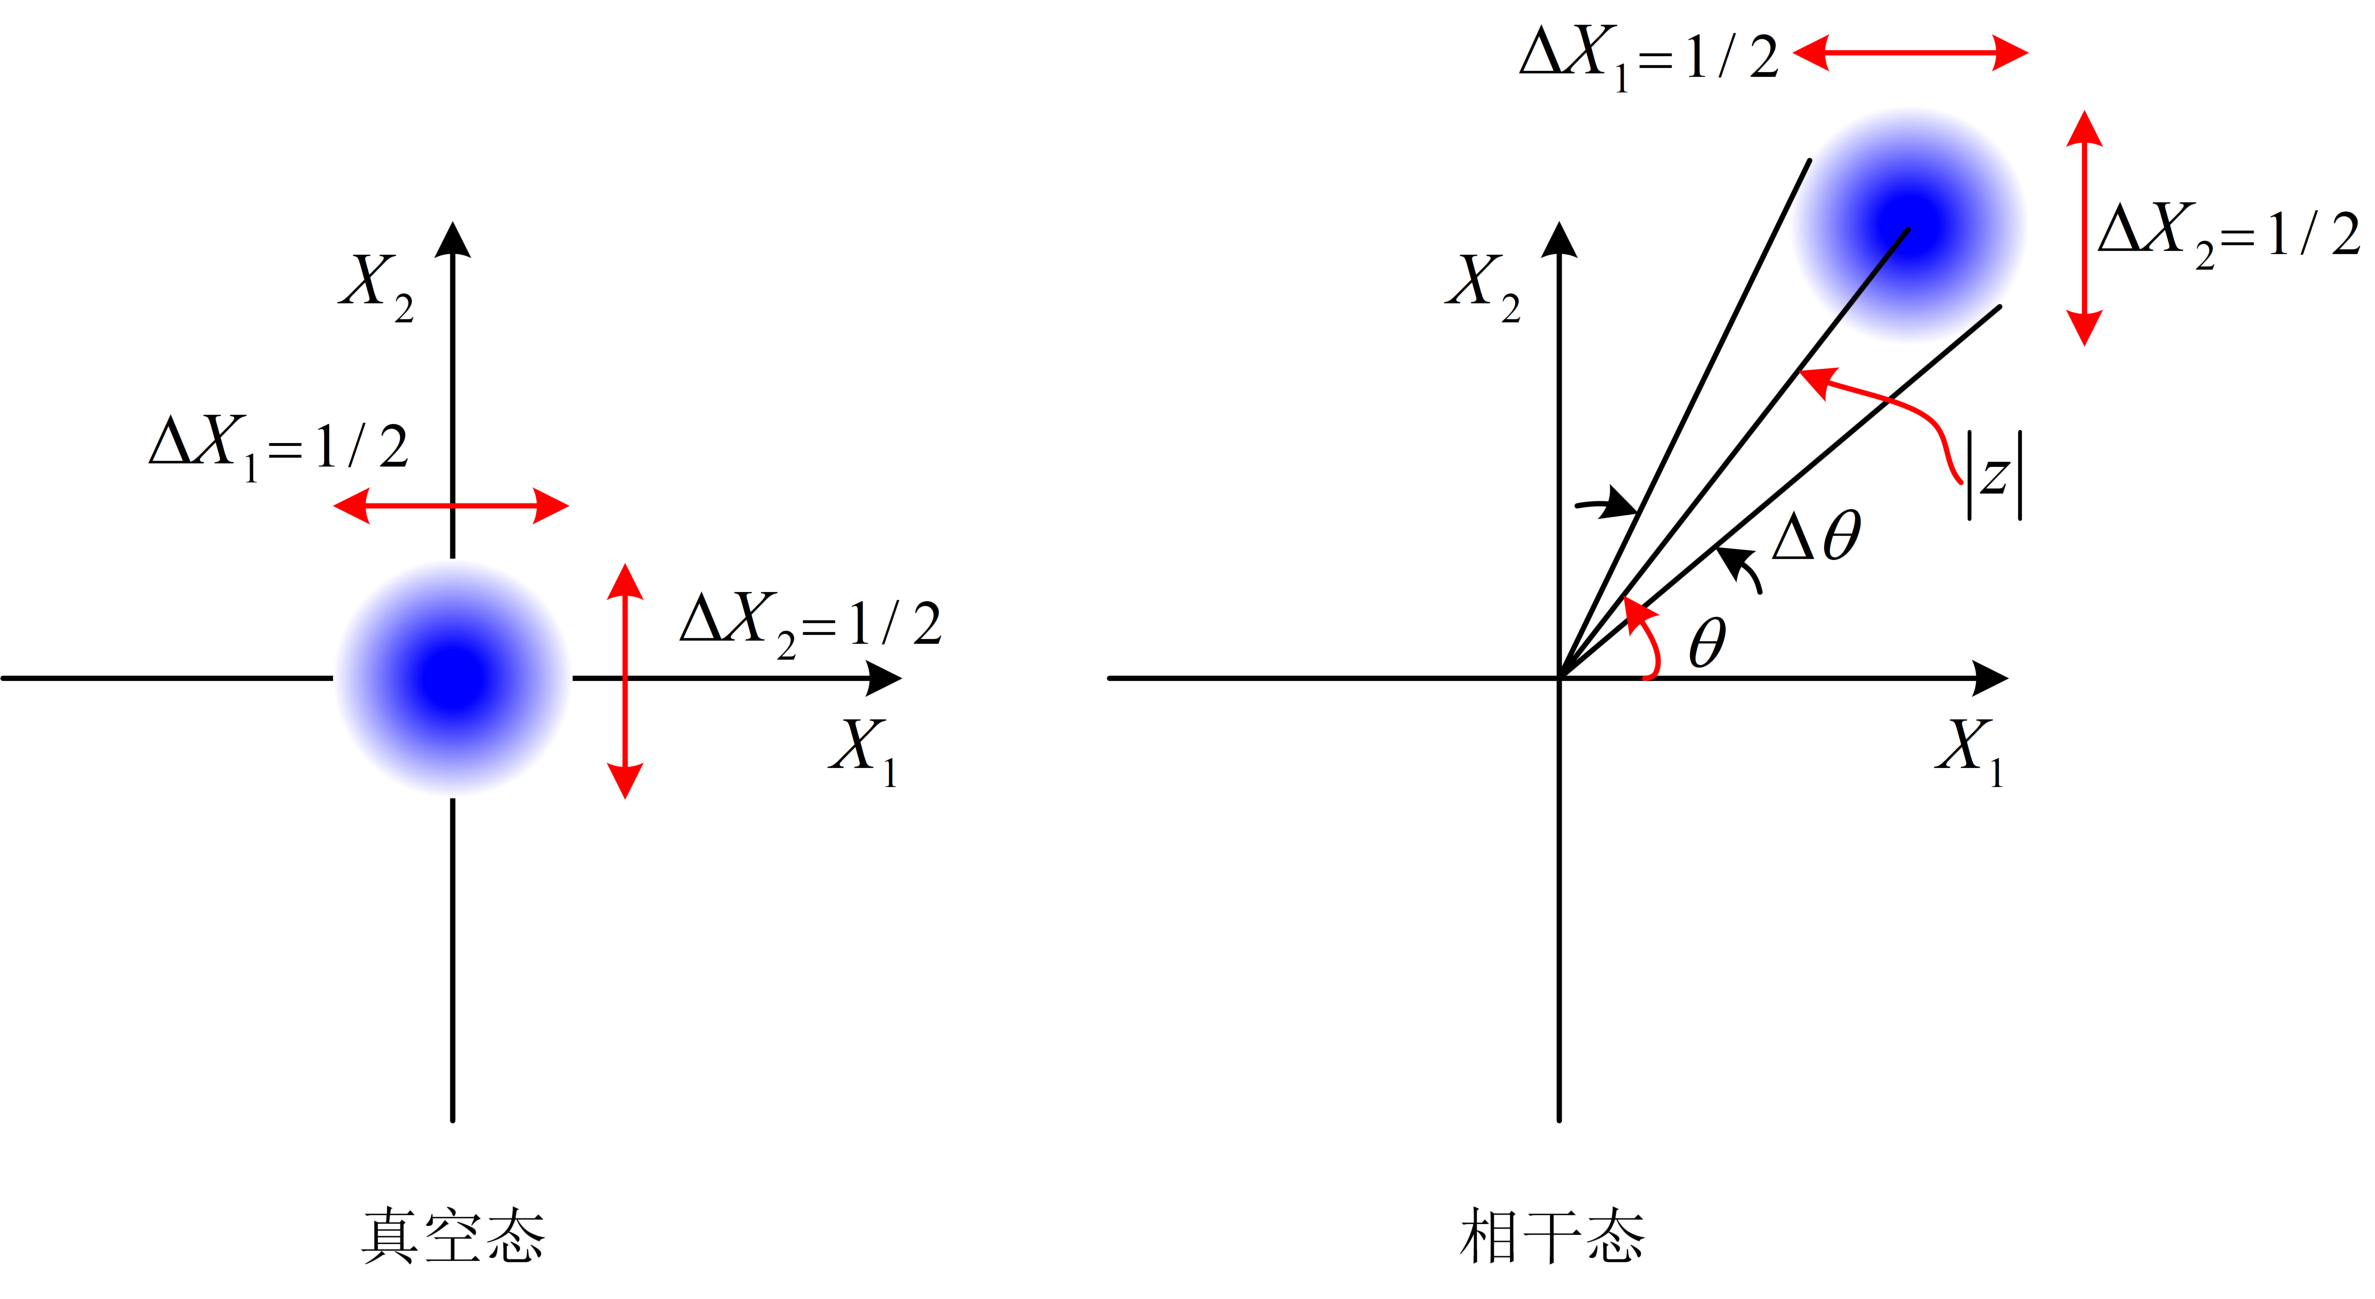
\includegraphics[width=0.8\textwidth]{L3/f1.pdf}
\caption{\justifying{正交分量在真空态和相干态中的涨落}}
\label{f1}
\end{figure}

\subsection{光的压缩态:量子涨落的减少}

\justifying{\setlength{\parindent}{2em}{从前面的讨论可知,真空态和相干态均为正交分量的最小不确定态,即在真空态和相干态中,电磁场正交算符$X_1$和$X_2$的标准偏差满足下式,即}
\begin{equation}
\Delta X_1=\dfrac{1}{2},\Delta X_2=\dfrac{1}{2},(\Delta X_1)(\Delta X_2)=\dfrac{1}{4}
\label{eq24}
\end{equation}

\justifying{\setlength{\parindent}{0em}{其中,$X_1=\dfrac{1}{2}(\hat{a}+\hat{a}^\dag),X_2=\dfrac{1}{2\text{i}}(\hat{a}-\hat{a}^\dag)$。}

\justifying{\setlength{\parindent}{2em}{由式(\ref{eq24})我们发现,根据量子理论一个电磁波的电场值不能以任何高的精度来预测,这是场的两个正交分量所满足的不确定关系的结果。不确定关系对它们方差的积施加了一个有限额度。该额度不仅仅是一个抽象的理论极限,它通常是决定高精密光学测量分辨率的最重要因素。这种情况下,光电探测器对场的测量出现了无法控制的源自量子性的涨落,称之为量子噪声\citep{ref3}。}

\justifying{\setlength{\parindent}{2em}{后来人们提出是否存在这样的一种量子态,在不违背不确定度关系$(\Delta X_1)(\Delta X_2)\geqslant1/4$的情况下,使得$\Delta X_i<1/2(i=1$或$2)$。在这样一个态的场中一个变量上表现出了量子噪声减少,代价是在另一个变量上噪声增加,对于增加光学测量可达精度而言,这样的态的潜力是不言而喻的。研究表明,这样的量子态是存在的,人们把这种量子态称为压缩态。}

\justifying{\setlength{\parindent}{2em}{Wigner函数是光场量子态在相空间的准几率分布函数,压缩态的性质通过Wigner函数更容易理解\citep{ref4},下图形象地展示了电场空间相关性的形式及场各种态((a)相干态、(b)正交振幅分量压缩的压缩态、(c)正交位相分量压缩的压缩态)的相量示意图。}
\begin{figure}[H]
\centering
	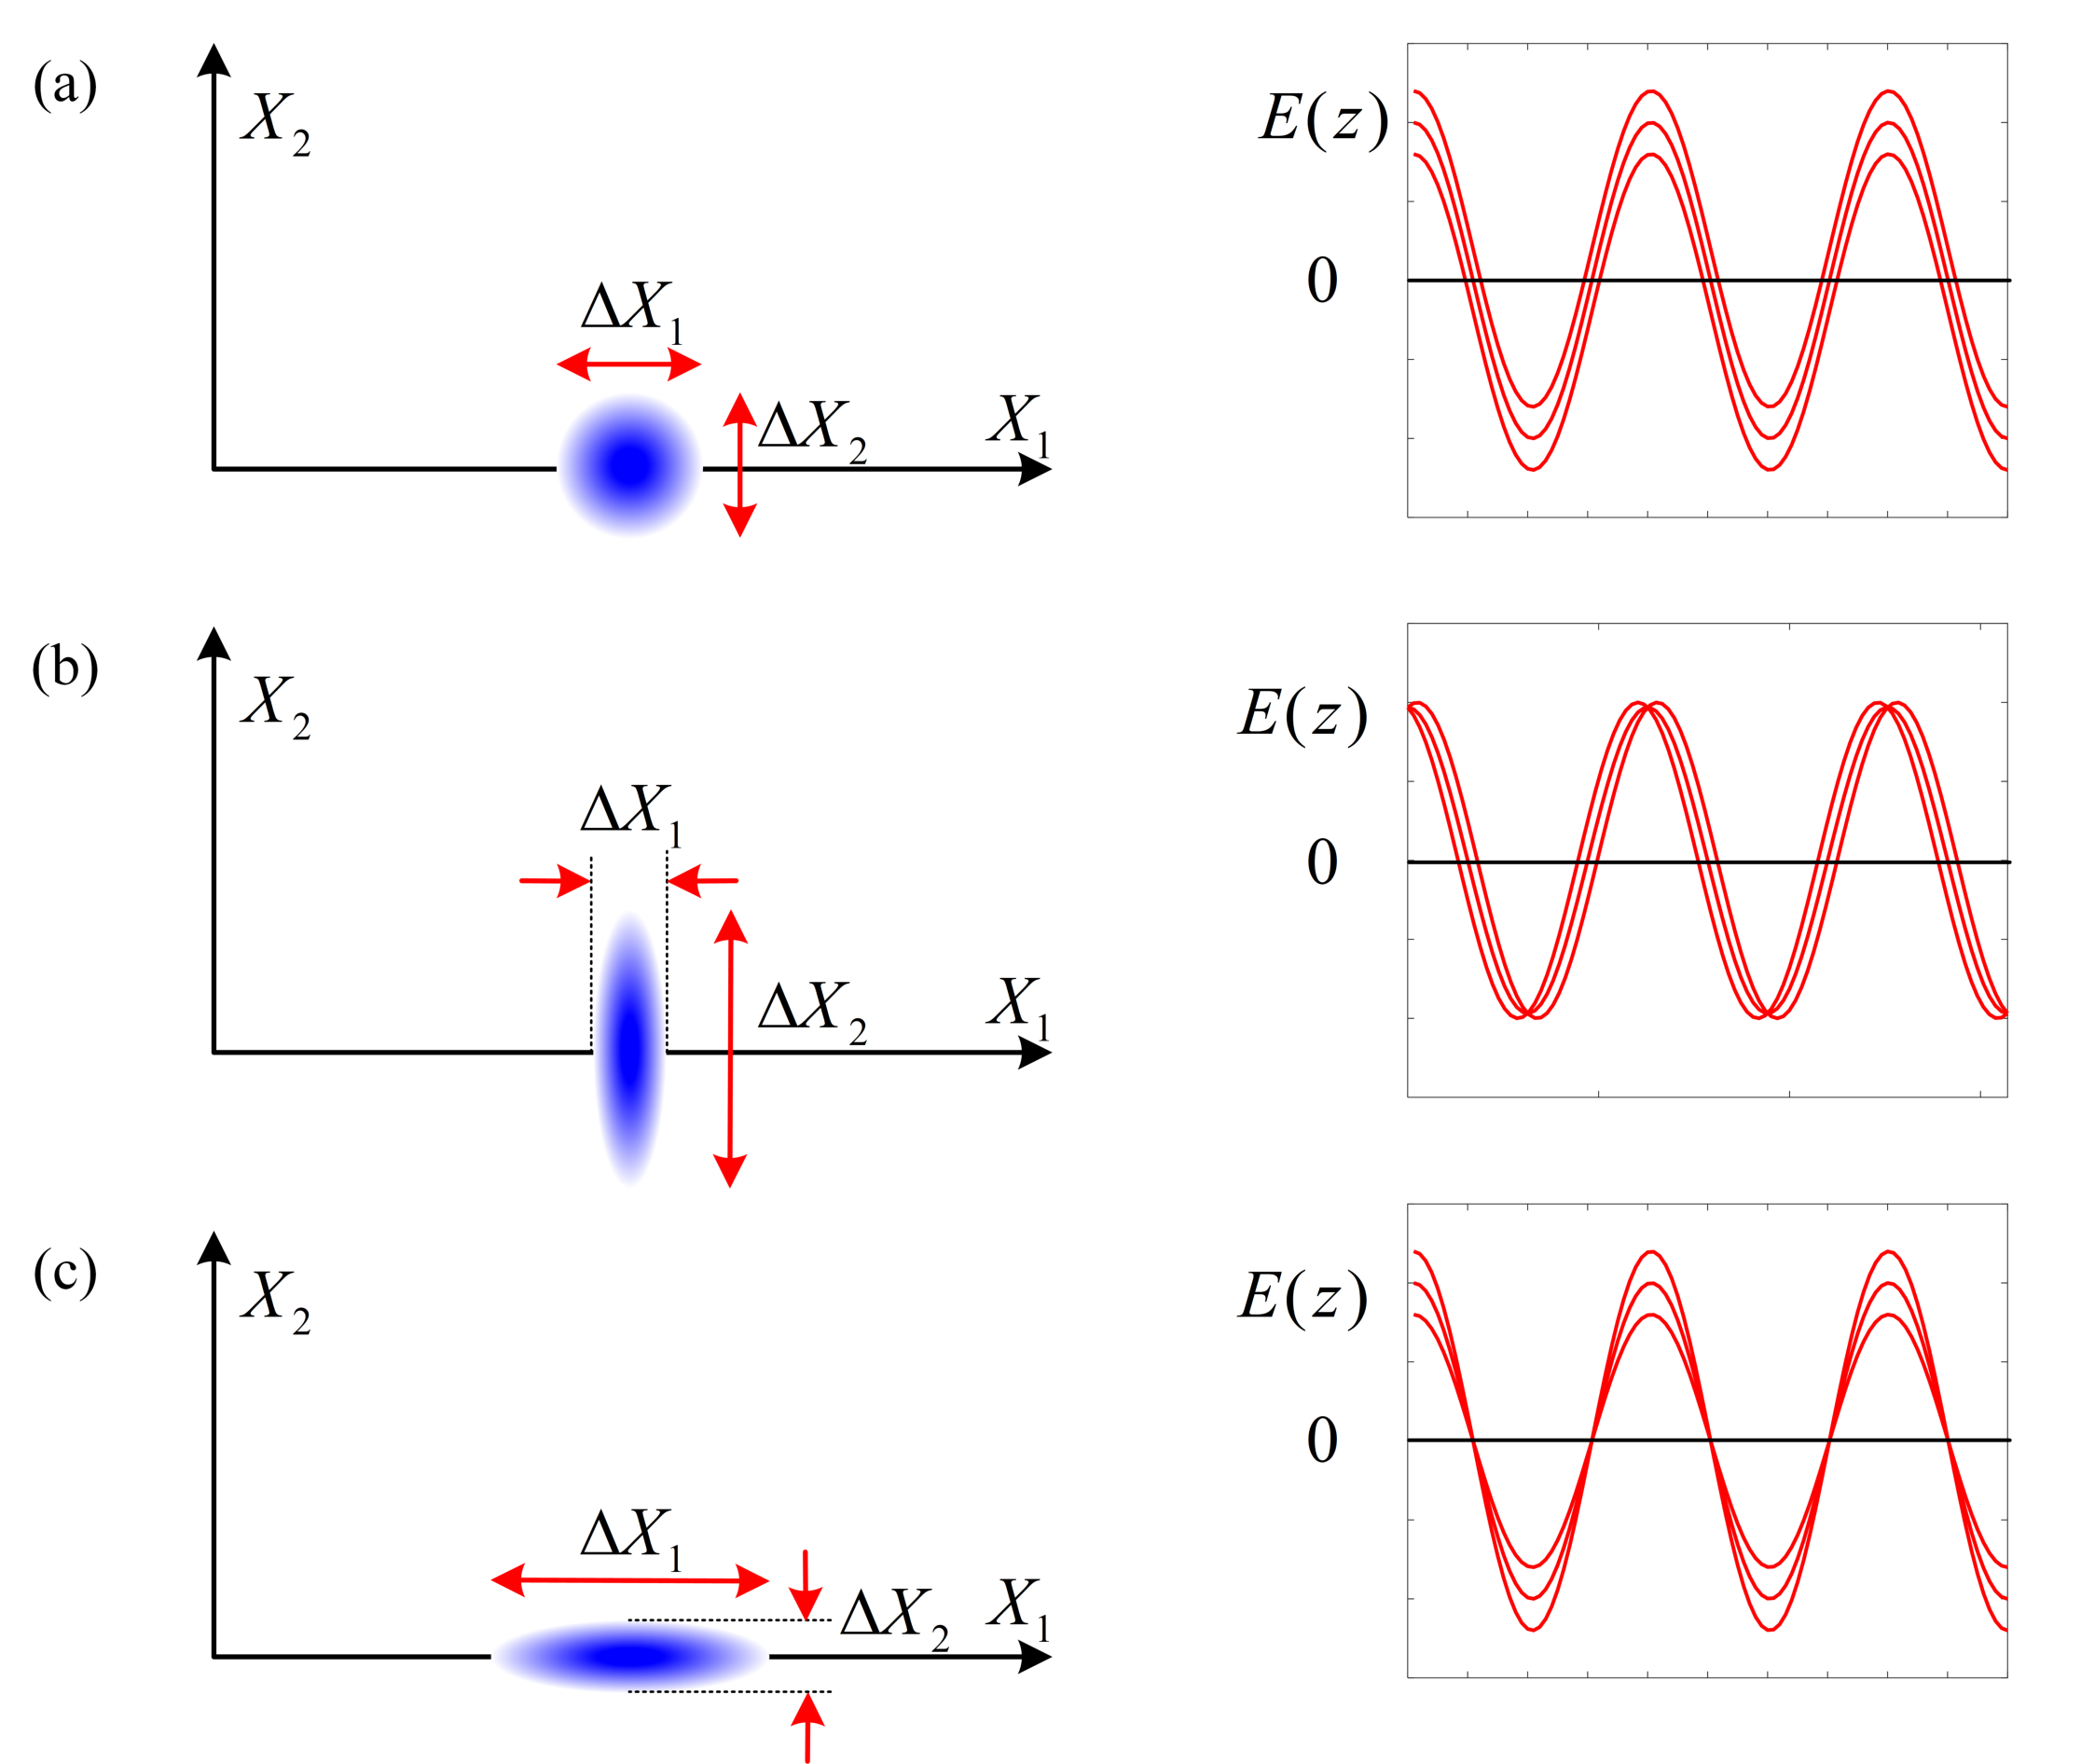
\includegraphics[width=0.8\textwidth]{L3/f2.pdf}
\caption{\justifying{电场空间相关性的形式及场各种态的相量表示}}
\label{f2}
\end{figure}

\justifying{\setlength{\parindent}{2em}{由上图可知,相干态下相量图是一个圆形区域,场是一个具有一定宽度的可能值的波带;在正交振幅分量压缩的压缩态下,在场的最大值处有很小的不确定性,而在零交叉处有最大的不确定性,此时场的振幅比相干态场的相位有更高的精度;在正交位相分量压缩的压缩态下,在场穿过零值的点上给出了一个减小的场的不确定性,而在场最大的点上给出了一个增加的不确定性,此时场的相位比相干态场的相位有更高的精度。}

\subsection{压缩真空态的平均光子数和光子数方差}

\justifying{\setlength{\parindent}{2em}{考虑压缩真空态(其名称可从下面讨论的性质看出),即}
\begin{equation}
\ket{\xi}=\hat{S}(\xi)\ket{0}
\label{eq25}
\end{equation}

\justifying{\setlength{\parindent}{0em}{其中}
\begin{equation}
\hat{S}(\xi)=\exp[\dfrac{1}{2}(\xi^*\hat{a}^2-\xi(\hat{a}^\dag)^2)]
\label{eq26}
\end{equation}

\justifying{\setlength{\parindent}{0em}{称为压缩算符;$\xi=r\text{e}^{\text{i}\theta}$},$\xi$称为压缩参量;$0\leqslant r<\infty$,称为压缩幅,描述压缩的强弱;$0\leqslant \theta<2\pi$,称为压缩角,描述压缩的方向。}

\justifying{\setlength{\parindent}{2em}{压缩算符具有以下性质,即}
\begin{equation}
\begin{cases}
\hat{S}^\dag(\xi)=\hat{S}^{-1}(\xi)=\hat{S}(-\xi) \\
\hat{S}^\dag(\xi)\hat{a}\hat{S}(\xi)=\hat{a}\cosh r-\hat{a}^\dag\text{e}^{\text{i}\theta}\sinh r \\
\hat{S}^\dag(\xi)\hat{a}^\dag\hat{S}(\xi)=\hat{a}^\dag\cosh r-\hat{a}\text{e}^{-\text{i}\theta}\sinh r
\end{cases}
\label{eq31}
\end{equation}

\justifying{\setlength{\parindent}{2em}{压缩真空态中的平均光子数为:}
\begin{align}
\braket{n}&=\braket{\hat{a}^\dag\hat{a}}\nonumber\\
& = \braket{\xi|\hat{a}^\dag\hat{a}|\xi}\nonumber\\
& = \braket{0|\hat{S}^\dag\hat{a}^\dag\hat{a}\hat{S}|0}\nonumber\\
& = \braket{0|(\hat{S}^\dag\hat{a}^\dag\hat{S})(\hat{S}^\dag\hat{a}\hat{S})|0}\nonumber\\
& = \braket{0|(\hat{a}^\dag\cosh r-\hat{a}\text{e}^{-\text{i}\theta}\sinh r)(\hat{a}\cosh r-\hat{a}^\dag\text{e}^{\text{i}\theta}\sinh r)|0}\nonumber\\
& = \sinh^2r
\label{eq32}
\end{align}
\begin{align}
\braket{n^2}&=\braket{(\hat{a}^\dag\hat{a})^2}\nonumber\\
& = \braket{\xi|\hat{a}^\dag\hat{a}\hat{a}^\dag\hat{a}|\xi}\nonumber\\
& = \braket{0|\hat{S}^\dag\hat{a}^\dag\hat{a}\hat{a}^\dag\hat{a}\hat{S}|0}\nonumber\\
& = \braket{0|(\hat{S}^\dag\hat{a}^\dag\hat{S})(\hat{S}^\dag\hat{a}\hat{S})(\hat{S}^\dag\hat{a}^\dag\hat{S})(\hat{S}^\dag\hat{a}\hat{S})|0}\nonumber\\
& = 2\sinh^2r\cosh^2r+\sinh^4r
\label{eq33}
\end{align}
\justifying{\setlength{\parindent}{2em}{所以压缩真空态中的光子数方差为:}
\begin{align}
V(n)=\braket{n^2}-\braket{n}^2=2\sinh^2r\cosh^2r=2\braket{n}(1+\braket{n})>\braket{n}
\label{eq34}
\end{align}

\justifying{\setlength{\parindent}{2em}{在这里引入Mandel Q参数,即}
\begin{align}
Q=\dfrac{V(n)}{\braket{n}}-1
\label{eq35}
\end{align}

\justifying{\setlength{\parindent}{0em}{若对某种光场态有$Q=0$,则光子数服从泊松分布;若$Q>0$,则光子数服从超泊松分布;若$Q<0$,则光子数服从亚泊松分布。显然由式(\ref{eq34})可知,压缩态的光子数分布呈现超泊松分布。}

\subsection{压缩真空态正交算符的平均值与方差}

\justifying{\setlength{\parindent}{2em}{接下来计算压缩真空态中正交算符的平均值和方差。}
\begin{equation}
X_1=\dfrac{1}{2}(\hat{a}+\hat{a}^\dag),X_2=\dfrac{1}{2\text{i}}(\hat{a}-\hat{a}^\dag)\nonumber
\end{equation}
\begin{equation}
X_1^2=\dfrac{1}{4}[(2\hat{a}^\dag\hat{a}+1)+(\hat{a}^2+(\hat{a}^\dag)^2)]\nonumber
\end{equation}
\begin{equation}
X_2^2=\dfrac{1}{4}[(2\hat{a}^\dag\hat{a}+1)-(\hat{a}^2+(\hat{a}^\dag)^2)]\nonumber
\end{equation}
\begin{equation}
\braket{X_1}=\dfrac{1}{2}(\braket{\hat{a}}+\text{C.C.}),\braket{X_2}=\dfrac{1}{2\text{i}}(\braket{\hat{a}}-\text{C.C.})
\label{eq36}
\end{equation}
\begin{equation}
\braket{X_1^2}=\dfrac{1}{4}[(2\braket{\hat{a}^\dag\hat{a}}+1)+(\braket{\hat{a}^2}+\text{C.C.})]\nonumber
\end{equation}
\begin{equation}
\braket{X_2^2}=\dfrac{1}{4}[(2\braket{\hat{a}^\dag\hat{a}}+1)-(\braket{\hat{a}^2}+\text{C.C.})]\nonumber
\end{equation}
\begin{equation}
V(X_i)=\braket{X_i^2}-\braket{X_i}^2
\label{eq37}
\end{equation}

\justifying{\setlength{\parindent}{2em}{压缩态下$\braket{\hat{a}}$为}
\begin{equation}
\braket{\hat{a}}=\braket{\xi|\hat{a}|\xi}=\braket{0|\hat{S}^\dag\hat{a}\hat{S}|0}=\braket{0|(\hat{a}\cosh r-\hat{a}^\dag\text{e}^{\text{i}\theta}\sinh r)|0}=0\nonumber
\end{equation}

\justifying{\setlength{\parindent}{2em}{压缩态下$\braket{\hat{a}^2}$为}
\begin{align}
\braket{\hat{a}^2}&=\braket{\xi|\hat{a}\hat{a}|\xi}\nonumber\\
&=\braket{0|\hat{S}^\dag\hat{a}\hat{S}\hat{S}^\dag\hat{a}\hat{S}|0}\nonumber\\
&=\braket{0|(\hat{a}\cosh r-\hat{a}^\dag\text{e}^{\text{i}\theta}\sinh r)(\hat{a}\cosh r-\hat{a}^\dag\text{e}^{\text{i}\theta}\sinh r)|0}\nonumber\\
&=-\cosh r\cdot\text{e}^{\text{i}\theta}\sinh r\nonumber
\end{align}

\justifying{\setlength{\parindent}{0em}{且有}
\begin{equation}
(\braket{\hat{a}^2}+\text{C.C.})=-2\cosh r\cdot\sinh r\cdot\cos\theta \nonumber
\end{equation}
\begin{equation}
\braket{\hat{a}^\dag\hat{a}}=\sinh^2r \nonumber
\end{equation}

\justifying{\setlength{\parindent}{2em}{将以上结果代入式(\ref{eq36})、式(\ref{eq37}),可得}
\begin{equation}
\braket{X_1}=\braket{X_2}=0 
\label{eq38}
\end{equation}

\justifying{\setlength{\parindent}{0em}{电磁场正交振幅算符$X_1$的方差为:}
\begin{equation}
V(X_1)=\dfrac{1}{4}(\cosh^2r+\sinh^2r-2\sinh r\cosh r\cos\theta)=\dfrac{1}{4}(2\sinh^2r+1-2\sinh r\cosh r\cos\theta)
\label{eq39}
\end{equation}

\justifying{\setlength{\parindent}{0em}{电磁场正交位相算符$X_2$的方差为:}
\begin{equation}
V(X_2)=\dfrac{1}{4}(\cosh^2r+\sinh^2r+2\sinh r\cosh r\cos\theta)=\dfrac{1}{4}(2\sinh^2r+1+2\sinh r\cosh r\cos\theta)
\label{eq40}
\end{equation}

\justifying{\setlength{\parindent}{2em}{为了描述在一般方向上的压缩,引入下列旋转正交分量,即}
\begin{equation}
\begin{cases}
Y_1 = \cos\dfrac{\theta}{2}X_1+\sin\dfrac{\theta}{2}X_2 \\
Y_2 = -\sin\dfrac{\theta}{2}X_1+\cos\dfrac{\theta}{2}X_2
\end{cases}
\label{eq41}
\end{equation}

\justifying{\setlength{\parindent}{0em}{计算可得,在压缩真空态中,算符$Y_1$和$Y_2$的平均值和标准偏差分别为}
\begin{equation}
\begin{cases}
\braket{Y_1}=\braket{Y_2}=0\\
\Delta Y_1=\dfrac{1}{2}\text{e}^{-r},\Delta Y_2=\dfrac{1}{2}\text{e}^{r},(\Delta Y_1)(\Delta Y_2)=\dfrac{1}{4}
\end{cases}
\label{eq42}
\end{equation}

\justifying{\setlength{\parindent}{0em}{可见,压缩真空态也是最小不确定度态(尽管不要求一般压缩态是最小不确定度态\citep{ref5})。$Y_1$和$Y_2$的量子涨落在相空间如图(\ref{f3})所示。}
\begin{figure}[H]
\centering
	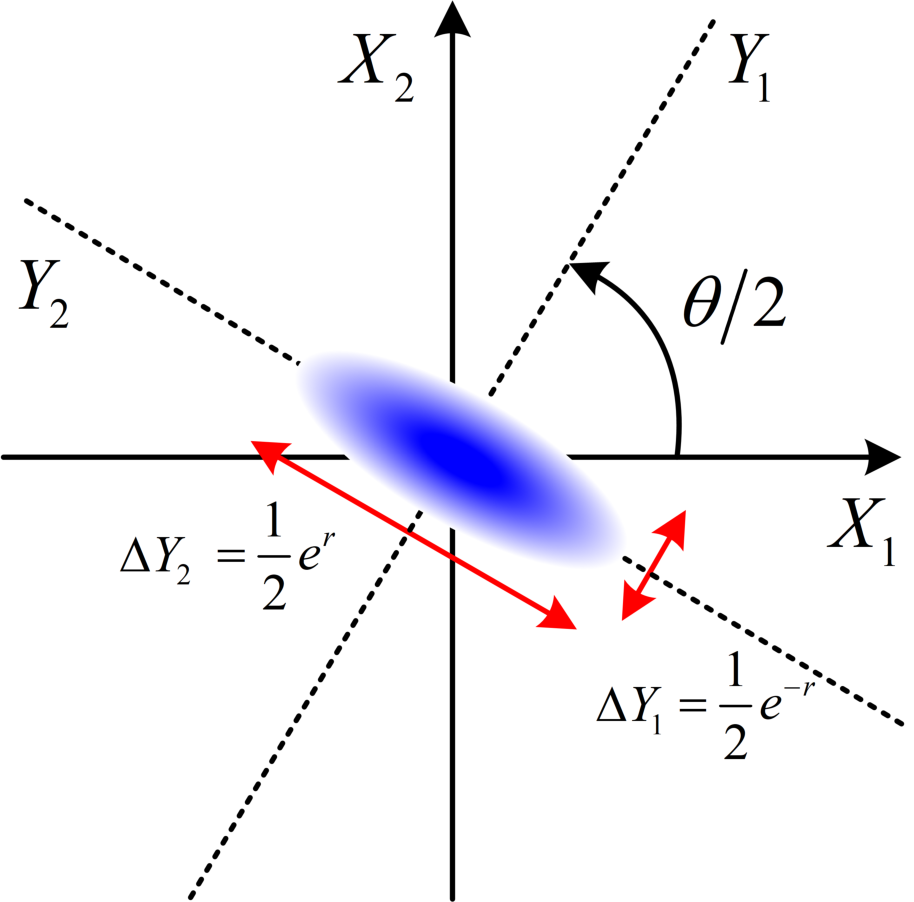
\includegraphics[width=0.3\textwidth]{L3/f3.pdf}
\caption{\justifying{旋转正交分量的涨落压缩}}
\label{f3}
\end{figure}

\subsection{压缩真空态的光子数分布}

\justifying{\setlength{\parindent}{2em}{由于$\hat{a}\ket{0}=0$,故对该式左乘$\hat{S}(\xi)$,$\hat{a}$右边添加一项$\hat{S}^\dag(\xi)\hat{S}(\xi)$,得}
\begin{equation}
\hat{S}(\xi)\hat{a}\hat{S}^\dag(\xi)\hat{S}(\xi)\ket{0}=0
\label{eq43}
\end{equation}
\begin{equation}
(\hat{a}\cosh r+\hat{a}^\dag\text{e}^{\text{i}\theta}\sinh r)\ket{\xi}=0
\label{eq44}
\end{equation}

\justifying{\setlength{\parindent}{0em}{式(\ref{eq44})即是压缩真空态$\ket{\xi}$满足的本征方程。}

\justifying{\setlength{\parindent}{2em}{令$\mu=\cosh r$,$\nu=\text{e}^{\text{i}\theta}\sinh r$,将压缩真空态用光子数态展开,有$\ket{\xi}=\sum\limits_{n}C_n\ket{n}$,代入式(\ref{eq44}),有:}
\begin{align}
0 & = (\mu\hat{a}+\nu\hat{a}^\dag)\sum\limits_{n}C_n\ket{n} \\
  & = \sum\limits_{n}C_n(\mu\sqrt{n}\ket{n-1}+\nu\sqrt{n+1}\ket{n+1})\\
  & = \sum\limits_{n}[\mu\sqrt{n+1}C_{n+1}+\nu\sqrt{n}C_{n-1}]\ket{n}
\label{eq45}
\end{align}

\justifying{\setlength{\parindent}{0em}{要使上式成立,要求}
\begin{align}
\mu\sqrt{n+1}C_{n+1}+\nu\sqrt{n}C_{n-1}=0
\label{eq46}
\end{align}

\justifying{\setlength{\parindent}{0em}{即}
\begin{align}
C_{n+1} & = -\dfrac{\nu}{\mu}\sqrt{\dfrac{n}{n+1}}C_{n-1} \\
C_2     & = -\dfrac{\nu}{\mu}\sqrt{\dfrac{1}{2}}C_{0}\\
C_4     & = -\dfrac{\nu}{\mu}\sqrt{\dfrac{3}{4}}C_{2}=(-\dfrac{\nu}{\mu})^2\sqrt{\dfrac{3\cdot1}{4\cdot2}}C_0...\\
C_{2m}  & = (-\dfrac{\nu}{\mu})^m\sqrt{\dfrac{(2m-1)!!}{(2m)!!}}C_0,m\geqslant1
\label{eq47}
\end{align}

\justifying{\setlength{\parindent}{2em}{$C_0$由归一化条件确定,即系数平方之和为1,最终计算得到压缩真空态在光子数态表象中的表示为}
\begin{equation}
	\textcolor[rgb]{1,0,0}{\ket{\xi}=\sum\limits_{m=0}^\infty\dfrac{1}{\sqrt{\cosh r}}(-1)^m(\dfrac{1}{2}\text{e}^{\text{i}\theta}\tanh r)^m\dfrac{\sqrt{(2m)!}}{m!}\ket{2m}}
\label{eq48}
\end{equation}

\justifying{\setlength{\parindent}{2em}{可见,在单模压缩真空态中只可能探测到偶数个光子,这从压缩算符$\hat{S}(\xi)$的定义式(\ref{eq26})的形式不难理解,产生算符和湮灭算符只成对出现。当$r\ll1$时,式(\ref{eq48})可以写为$\ket{\xi}=\ket{0}+\dfrac{r}{\sqrt{2}}\ket{2}+O(r^2)$,可以看出,尽管真空态的平均光子数为0,而压缩真空态的平均光子数大于0。}

\subsection{平移压缩真空态和压缩相干态}

\justifying{\setlength{\parindent}{2em}{平移压缩真空态的定义为}
\begin{equation}
\ket{z,\xi}=\hat{D}(z)\hat{S}(\xi)\ket{0}=\hat{D}(z)\ket{\xi}
\label{eq54}
\end{equation}

\justifying{\setlength{\parindent}{2em}{当$z=0$时,平移压缩真空态变为压缩真空态,即}
\begin{equation}
\ket{0,\xi}=\hat{D}(0)\hat{S}(\xi)\ket{0}=\hat{S}(\xi)\ket{0}=\ket{\xi}
\label{eq55}
\end{equation}

\justifying{\setlength{\parindent}{2em}{当$\xi=0$时,平移压缩真空态变为相干态,即}
\begin{equation}
\ket{z,0}=\hat{D}(z)\hat{S}(0)\ket{0}=\hat{D}(z)\ket{0}=\ket{z}
\label{eq56}
\end{equation}

\justifying{\setlength{\parindent}{2em}{平移压缩真空态中的平均光子数为$\braket{n}=|z|^2+\sinh^2r$,旋转正交分量$Y_1$和$Y_2$的平均值分别为}
\begin{equation}
\begin{cases}
\braket{Y_1}=\dfrac{1}{2}(z\text{e}^{-\text{i}\theta/2}+z^*\text{e}^{\text{i}\theta/2})  \vspace{0.5em}\\
\braket{Y_2}=\dfrac{1}{2\text{i}}(z\text{e}^{-\text{i}\theta/2}-z^*\text{e}^{\text{i}\theta/2})
\end{cases}
\label{eq57}
\end{equation}
\begin{equation}
\Delta Y_1=\dfrac{1}{2}\text{e}^{-r},\Delta Y_2=\dfrac{1}{2}\text{e}^{r},(\Delta Y_1)(\Delta Y_2)=\dfrac{1}{4}
\label{eq58}
\end{equation}

\justifying{\setlength{\parindent}{2em}{平移真空压缩态的标准偏差与在压缩真空态中相同,仍满足式(\ref{eq58})。我们再次看到,平移算符只改变正交分量算符$Y_1$和$Y_2$在量子态中的平均值,而不改变涨落性质。平移压缩真空态和压缩相干态的$Y_1$和$Y_2$的量子涨落在相空间如图(\ref{f4})所示。}
\begin{figure}[H]
\centering
	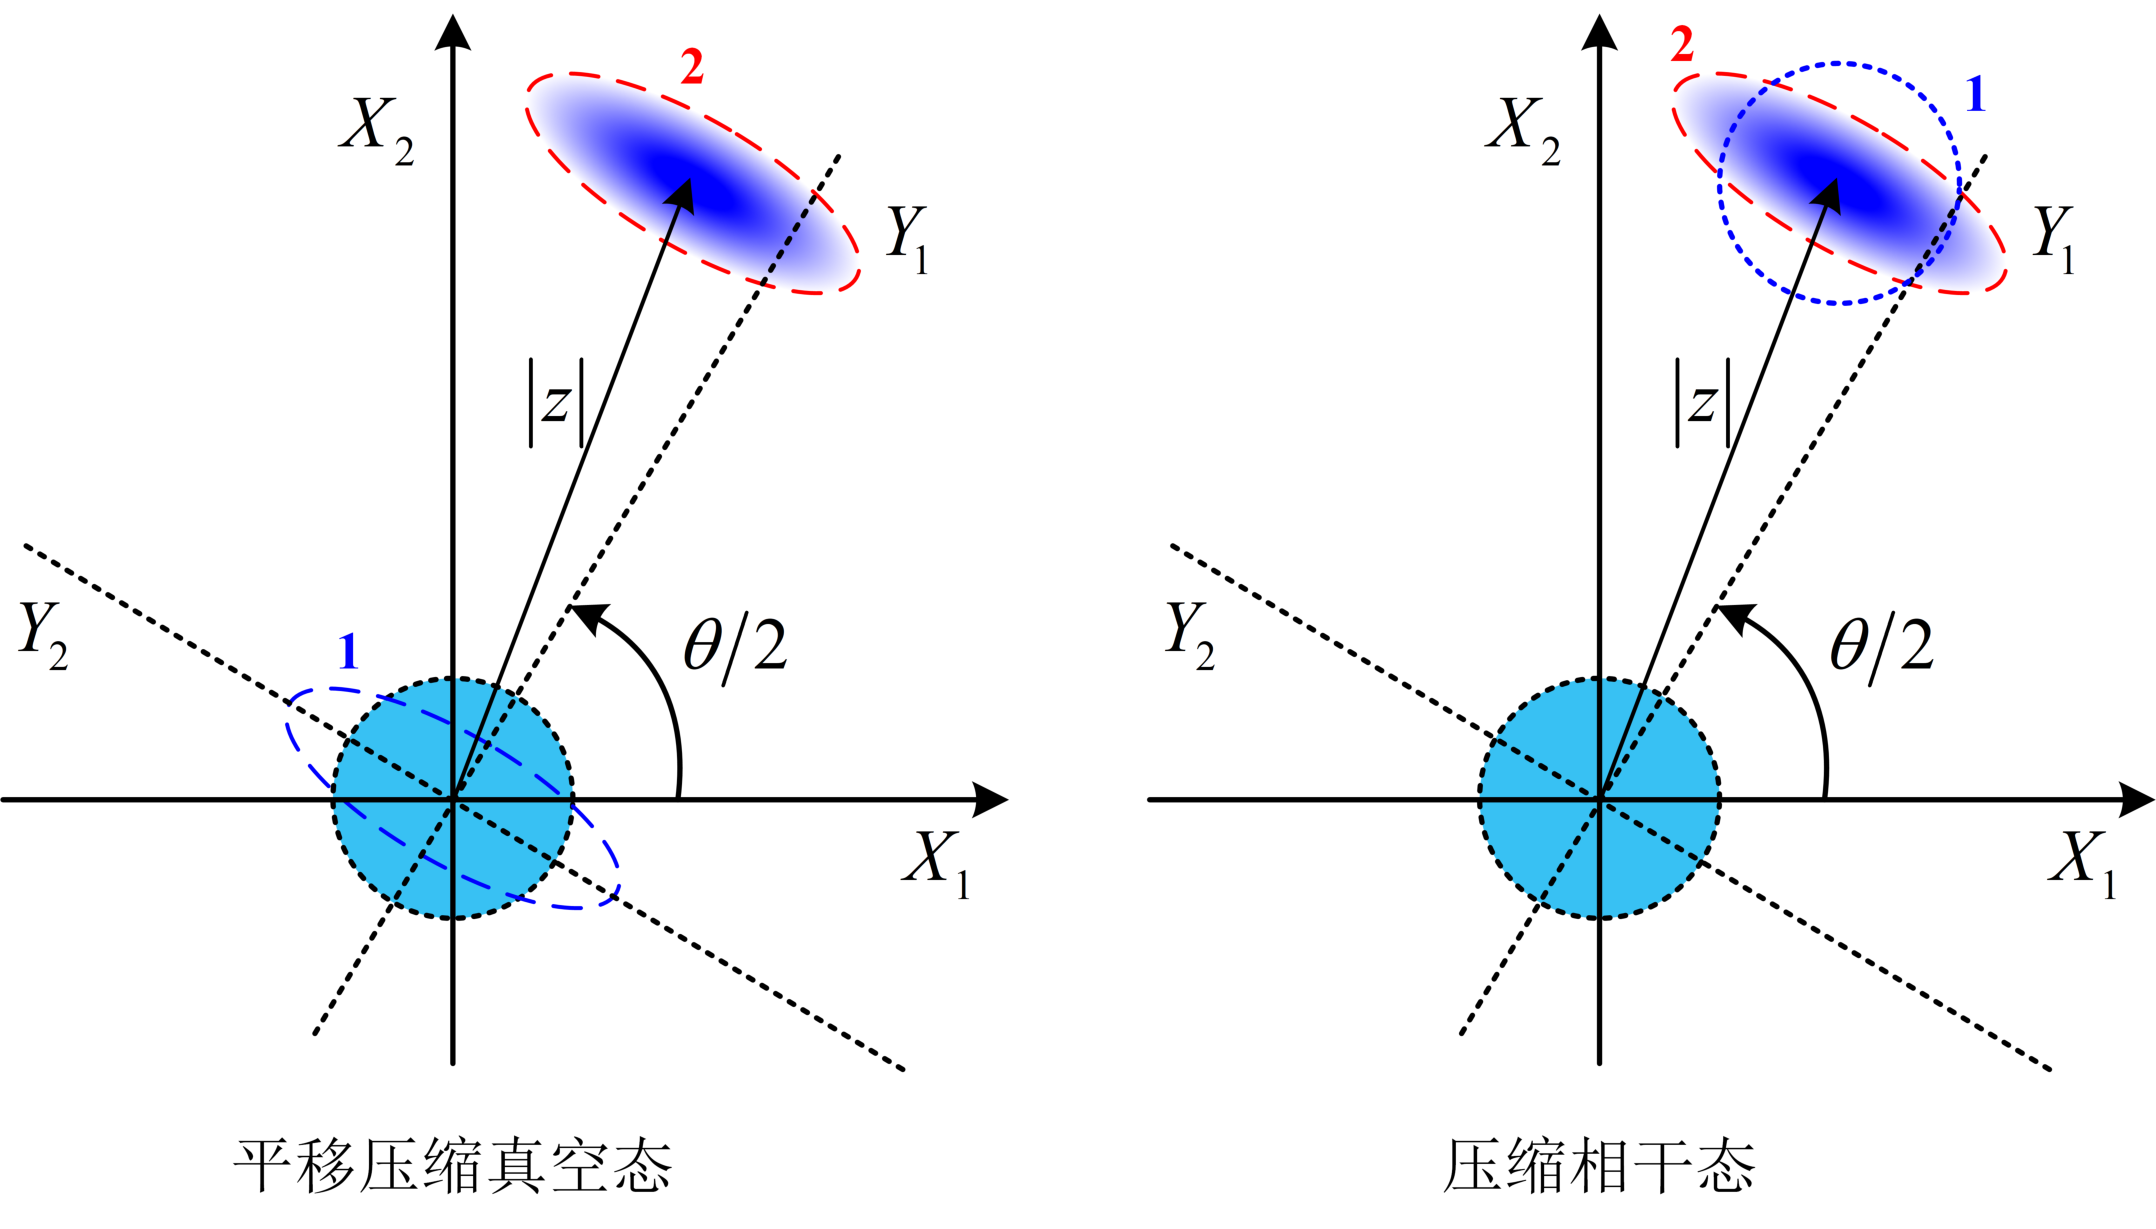
\includegraphics[width=0.8\textwidth]{L3/f4.pdf}
\caption{\justifying{旋转正交分量在平移压缩真空态和压缩相干态中的涨落压缩}}
\label{f4}
\end{figure}

\justifying{\setlength{\parindent}{2em}{压缩相干态(曾称为双光子相干态)定义为}
\begin{equation}
\hat{S}(\xi)\ket{z}=\hat{S}(\xi)\hat{D}(z)\ket{0}
\label{eq59}
\end{equation}

\justifying{\setlength{\parindent}{2em}{与平移压缩真空态比较,压缩算符和平移算符调换了次序(对应于两个物理过程的先后次序作了调换)。一般来说,压缩算符和平移算符互不对易,因此压缩相干态不等于平移压缩真空态,即}
\begin{equation}
\hat{S}(\xi)\ket{z}=\hat{S}(\xi)\hat{D}(z)\ket{0}\neq\hat{D}(z)\hat{S}(\xi)\ket{0}
\label{eq60}
\end{equation}

\justifying{\setlength{\parindent}{0em}{但是可以证明}
\begin{equation}
\hat{S}(\xi)\ket{\beta}=\hat{S}(\xi)\hat{D}(\beta)\ket{0}=\hat{D}(z)\hat{S}(\xi)\ket{0}
\label{eq61}
\end{equation}

\justifying{\setlength{\parindent}{0em}{其中,$\beta=\mu z+\nu z^*$。}

\justifying{\setlength{\parindent}{2em}{因此,经过适当的参数变换,压缩相干态可化作平移压缩真空态,从这个意义上来说,二者是等价的。}
%%%%%%%%%%%%%%%%%%%%%%%%%%%%%%%%%%%%%%%%%%%%%%%%%%%%%%%%%%%%%%%%%%%%%%%%%%%%%%%%%%%%%%%%%%%%%%%%%%%%%
\section{\large 压缩态光场的产生}

\justifying{\setlength{\parindent}{2em}{压缩真空态由式(\ref{eq25})和式(\ref{eq26})定义,即}
\begin{equation}
\ket{\xi}&=\hat{S}(\xi)\ket{0}
\label{eq62}
\end{equation}
\justifying{\setlength{\parindent}{0em}{和}
\begin{equation}
\hat{S}(\xi)=\exp[\dfrac{1}{2}&(\xi^*\hat{a}^2-\xi(\hat{a}^\dag)^2)]
\label{eq63}
\end{equation}

\justifying{\setlength{\parindent}{2em}{在量子力学中,量子态随时间的演化是幺正演化,即}
\begin{equation}
\ket{\psi(t)}=\hat{U}(t)\ket{\psi(0)}
\label{eq64}
\end{equation}

\justifying{\setlength{\parindent}{0em}{其中}
\begin{equation}
\hat{U}(t)=\exp(-\dfrac{\text{i}}{\hbar}\hat{H}t)
\label{eq65}
\end{equation}

\justifying{\setlength{\parindent}{0em}{是体系的时间演化算符,$\hat{H}$是体系的哈密顿量。}

\justifying{\setlength{\parindent}{2em}{设体系初始处于真空态,即$\ket{\psi(0)}=\ket{0}$,则式(\ref{eq64})变为}
\begin{equation}
\ket{\psi(t)}=\hat{U}(t)\ket{0}
\label{eq66}
\end{equation}

\justifying{\setlength{\parindent}{0em}{将式(\ref{eq66})与式(\ref{eq62})比较,可以发现,如果时间演化算符$\hat{U}(t)$具有压缩算符$\hat{S}(\xi)$的形式,则$t$时刻体系将处于压缩真空态。进一步比较式(\ref{eq63})与式(\ref{eq65}),发现如果体系的哈密顿量$\hat{H}$描述某种双光子过程,则该过程就可以产生压缩真空态。}

\justifying{\setlength{\parindent}{2em}{最常见的产生压缩态的方法是通过非线性光波混合过程实现的,在这个过程中成对的光子被发射成简并(单模压缩)或非简并(双模压缩)模式。}

\subsection{简并参量下转换}

\justifying{\setlength{\parindent}{2em}{飞秒或皮秒线宽的强泵浦光单次穿过一块二阶非线性晶体,泵浦光中的一个光子可以分裂成两个能量较低的光子。产生光子的频率、波矢和偏振由相位匹配条件决定。如果产生的两个光子是简并的,即其频率、方向和偏振等所有自
由度都是不可区分的,则产生单模压缩态。图(\ref{f5})为简并光学参量放大器。}
\begin{figure}[H]
\centering
	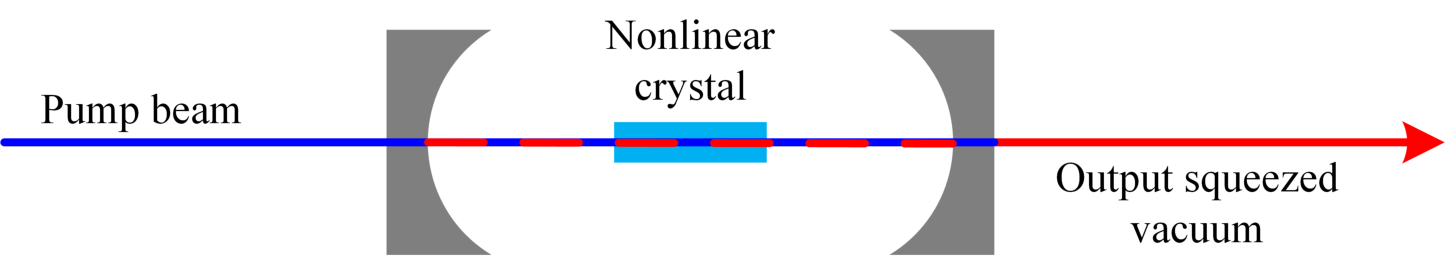
\includegraphics[width=0.8\textwidth]{L3/f5.pdf}
\caption{\justifying{简并光学参量放大器}}
\label{f5}
\end{figure}

\justifying{\setlength{\parindent}{2em}{描述简并参量下转换过程的哈密顿量为}
\begin{equation}
\hat{H}=\hbar\omega\hat{a}^\dag\hat{a}+\hbar\omega_p\hat{b}^\dag\hat{b}+\text{i}\hbar\chi^{(2)}[\hat{a}^2\hat{b}^\dag-(\hat{a}^\dag)^2\hat{b}]
\label{eq67}
\end{equation}

\justifying{\setlength{\parindent}{0em}{其中,$\omega$和$\hat{a}$分别是信号场的频率和光子湮灭算符;$\omega_p$和$\hat{b}$是泵浦场的频率和光子湮灭算符;$\chi^{(2)}$是实数,与二阶非线性极化率有关。}

\justifying{\setlength{\parindent}{2em}{一般来说,泵浦场越强,可作经典描述(称为参量近似),即令$\hat{b}\rightarrow\beta\text{e}^{-\text{i}\omega_pt}$。于是,哈密顿量可写为}

\begin{equation}
\hat{H}=\hbar\omega\hat{a}^\dag\hat{a}+\text{i}\hbar[\eta^*\text{e}^{\text{i}\omega_pt}\hat{a}^2-\eta\text{e}^{-\text{i}\omega_pt}(\hat{a}^\dag)^2]
\label{eq68}
\end{equation}

\justifying{\setlength{\parindent}{0em}{其中,$\eta=\chi^{(2)}\beta$。}

\justifying{\setlength{\parindent}{2em}{变换到相互作用绘景,$\hat{a}\rightarrow\hat{a}\text{e}^{-\text{i}\omega t}$,则在相互作用绘景中的相互作用哈密顿量为(同时考虑共振情况$\omega_p=2\omega$)}

\begin{equation}
\hat{H}_I=\text{i}\hbar[\eta^*\hat{a}^2-\eta(\hat{a}^\dag)^2]
\label{eq69}
\end{equation}

\justifying{\setlength{\parindent}{0em}{于是有}

\begin{equation}
\hat{U}(t)=\exp(-\dfrac{\text{i}}{\hbar}\hat{H}_It)=\exp[t\eta^*\hat{a}^2-t\eta(\hat{a}^\dag)^2]
\label{eq70}
\end{equation}

\justifying{\setlength{\parindent}{0em}{将式(\ref{eq70})与式(\ref{eq63})比较,发现若令$\xi=2t\eta=2t\chi^{(2)}\beta$,则$\hat{U}(t)=\hat{S}(\xi)$。于是,当体系初始处于真空态时,$t$时刻体系将演化到压缩真空态。}

\subsection{简并四波混频}

\justifying{\setlength{\parindent}{2em}{2008年,美国国家标准技术局的Lett教授课题组利用基于铷原子系综中双Λ型能级结构的四波混频过程制备了双模压缩态,随后将其推广至简并四波混频过程制备了单模压缩态\citep{ref6}。原子系综中的四波混频对应的光束结构和能级过程如图(\ref{f6})所示。}

\begin{figure}[H]
\centering
	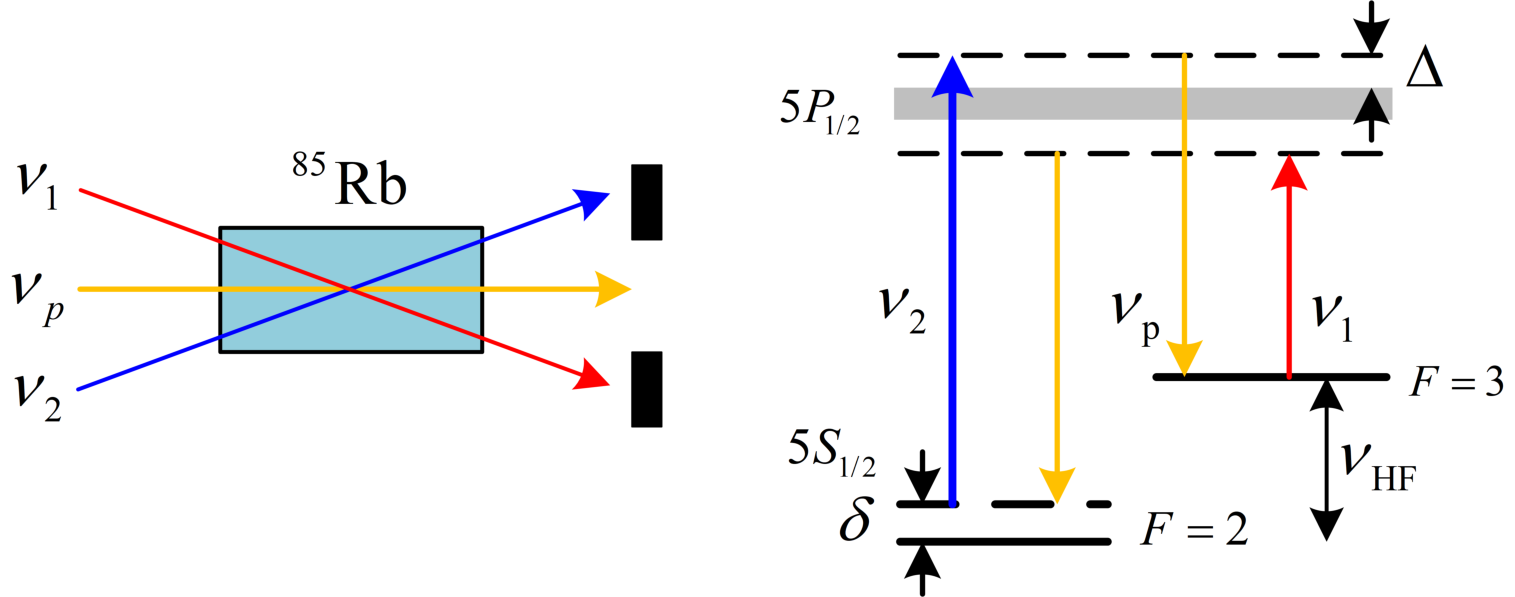
\includegraphics[width=0.6\textwidth]{L3/f6.pdf}
\caption{\justifying{简并情况下得到单模压缩态\citep{ref6}}}
\label{f6}
\end{figure}

\justifying{\setlength{\parindent}{2em}{与利用二阶非线性效应的自发参量下转换不同的是,四波混频过程利用的是原子系综的三阶非线性效应。在四波混频过程中,两个泵浦光子转换为两个信号光子,该过程满足能量守恒与动量守恒。描述简并四波混频过程的哈密顿量为}
\begin{equation}
\hat{H}=\hbar\omega\hat{a}^\dag\hat{a}+\hbar\omega_p\hat{b}^\dag\hat{b}+\text{i}\hbar\chi^{(3)}[\hat{a}^2(\hat{b}^\dag)^2-(\hat{a}^\dag)^2\hat{b}^2]
\label{eq71}
\end{equation}

\justifying{\setlength{\parindent}{0em}{其中,$\chi^{(3)}$是实数,与三阶非线性极化率有关。}

\justifying{\setlength{\parindent}{2em}{与简并参量下转换过程作类似的讨论,取参量近似,变换到相互作用绘景、考虑共振情况$\omega_p=\omega$,则可得到与式(\ref{eq69})形式相同的公式,只需将$\eta=\chi^{(2)}\beta$换成$\eta=\chi^{(3)}\beta^2$。}
%%%%%%%%%%%%%%%%%%%%%%%%%%%%%%%%%%%%%%%%%%%%%%%%%%%%%%%%%%%%%%%%%%%%%%%%%%%%%%%%%%%%%%%%%%%%%%%%%%%%%
\section{\large 压缩态的应用}

\subsection{干涉测量:提高激光干涉引力波探测的灵敏度}

\justifying{\setlength{\parindent}{2em}{大多数标准测量技术的测量精度由一些可避免的误差来源限制。最典型的例子是影响电磁场振幅测量的真空波动的环境感生噪声(散粒噪声)和自由粒子位移测量中的动态感生噪声(标准量子极限)。散粒噪声和标准量子极限给测量精度设立了一个重要基准,也给试图打败这个基准的科学家们提供了一个巨大挑战。直到量子力学的出现,突破经典测量方法的极限成为了可能。利用非经典光场注入干涉仪测量技术就是其中一种有力的突破散粒噪声极限,提高测量灵敏度的方法。}

\justifying{\setlength{\parindent}{2em}{1981年,Caves从理论上证明了把压缩光注入干涉仪能够提高系统灵敏度。Caves设想了一种方法能测量到在散粒噪声基准以下的信号,类似于干涉仪的量子力学仪器对信号的响应显示,所有测量到的噪声来自于通过50:50分束器端口进入干涉仪的真空场的一个正交态\citep{ref7}。Caves的想法是用一个压缩态来代替真空态,因为压缩态在这个正交处噪声较低,所以降低了量子噪声,从而增加了信噪比。}

\justifying{\setlength{\parindent}{2em}{MZ干涉仪是一种典型的高灵敏度干涉仪测量装置,利用压缩态光场注入干涉仪提高其灵敏度的实验原理图如下图(\ref{f7})所示:本底光场$a$和压缩真空态$b$同时注入BS之后,分成反射光和透射光,这两部分光沿着不同路径传播,最终在第二个BS处重合,通过测量两个输出场的强度就可以监视两个模式$c$和$d$的位相差$\phi$。}
\begin{figure}[H]
\centering
	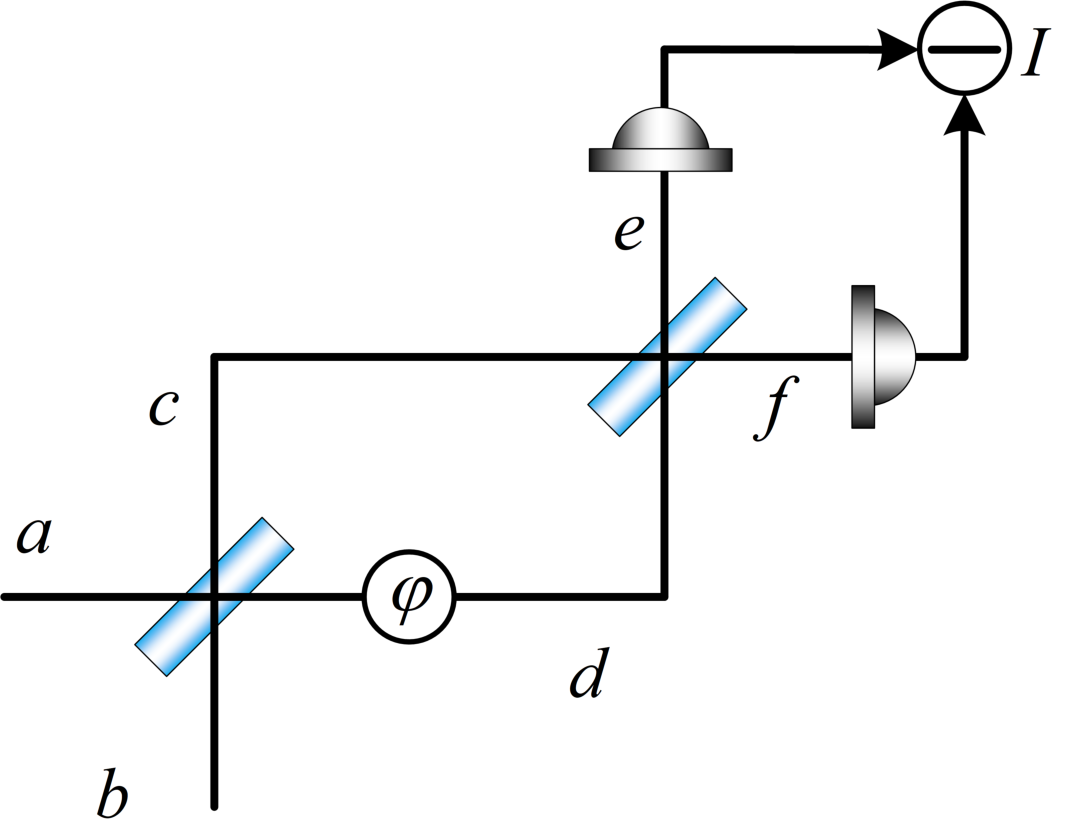
\includegraphics[width=0.4\textwidth]{L3/f7.pdf}
\caption{\justifying{马赫-增德尔干涉仪示意图}}
\label{f7}
\end{figure}

\justifying{\setlength{\parindent}{2em}{干涉仪探测原理是基于分析光电流中的位相变化,位相$\phi$的任意变化$\Delta\phi$会导致$\hat{I}(\phi)$值的变化,通过理论计算\citep{ref8},可得如果只注入本底光场,则总光子数$N=Z^2$,这时$\Delta\phi=N^{-1/2}$,即散粒噪声极限;同时注入本底光场和压缩真空态时,$\Delta\phi$的最小值$N^{-3/4}<N^{-1/2}$,小于散粒噪声极限。图(\ref{f8})左图展示了量子增强型光纤干涉仪实验装置图,右图展示了DOPO腔输出的压缩光噪声谱,可以看到压缩态光的注入使得噪声低于SNL。}

\begin{figure}[H]
\centering
	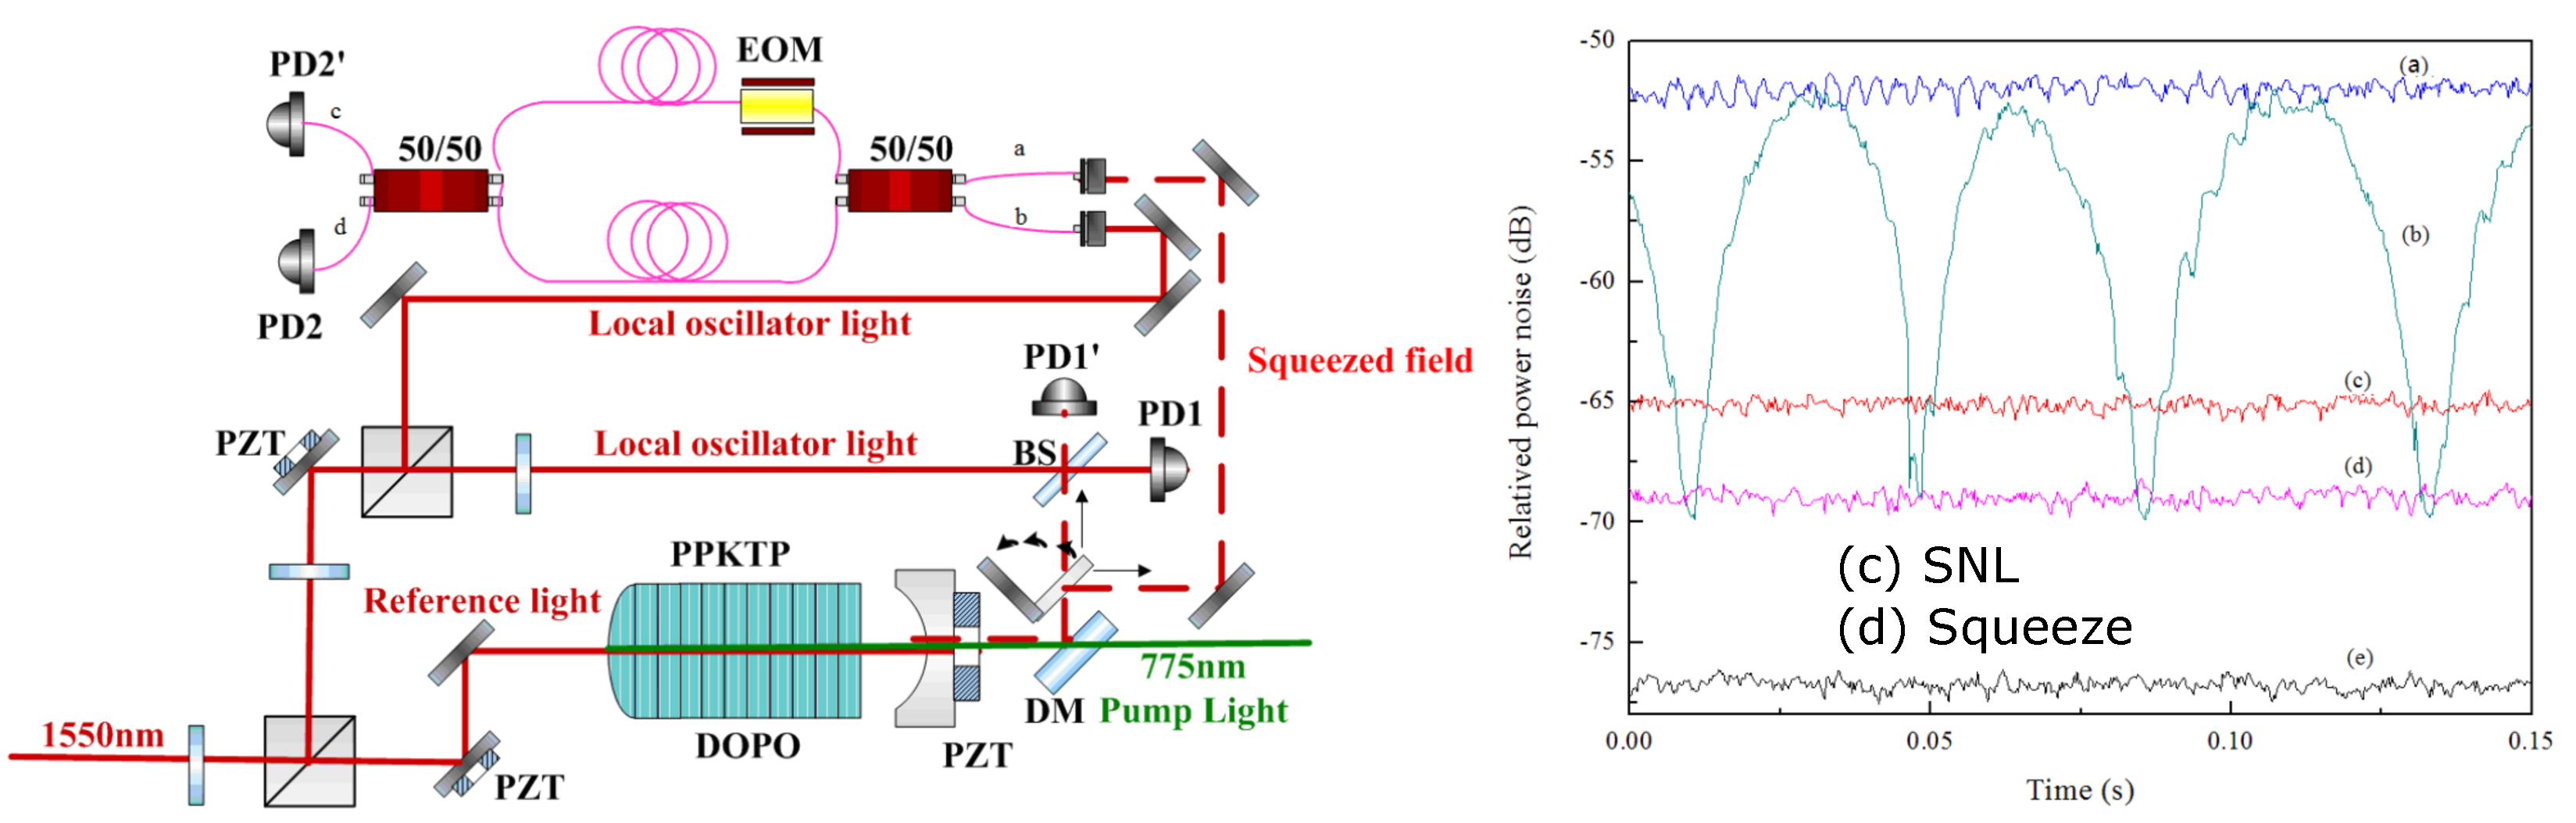
\includegraphics[width=\textwidth]{L3/f8.pdf}
\caption{\justifying{压缩态光场注入光纤干涉仪进行突破散粒噪声极限精密测量\citep{ref8}}}
\label{f8}
\end{figure}

\justifying{\setlength{\parindent}{2em}{20世纪90年代,美国开始在相距3000km的华盛顿州和路易斯安那州同时建设两台臂长达到4km的L型激光干涉引力波探测器(LIGO),之后并不断对其进行升级。直到2015年9月,LIGO首次探测到了引力波信号。LIGO的基本模型为光学迈克尔逊干涉仪,引力波因其干涉仪其中一臂长度增加,另一臂长度减小,因此对应干涉仪输出的功率发生相应变化。LIGO使用了高真空度、多级隔振、功率循环腔、高功率激光等技术来提高灵敏度。在将各种经典噪声降低至最低之后,将正交位相分量压缩态光场注入激光干涉引力波探测器的暗端口,其灵敏度可以进一步提高\citep{ref9}。}
\begin{figure}[H]
\centering
	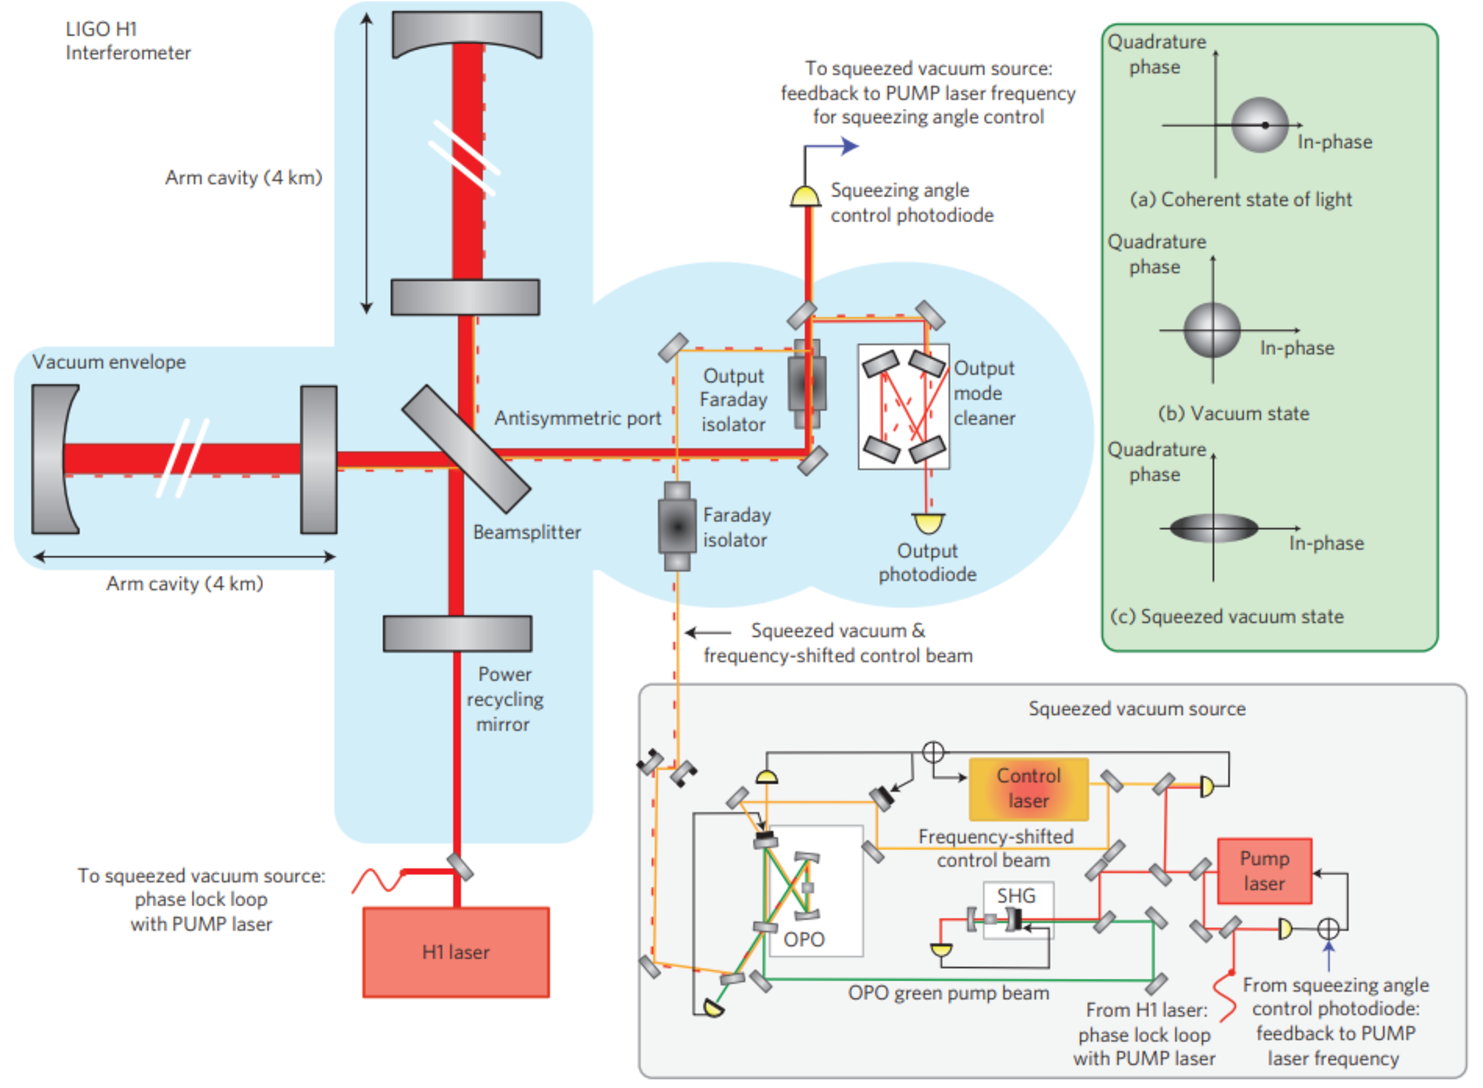
\includegraphics[width=0.8\textwidth]{L3/f9.pdf}
\caption{\justifying{压缩态光场注入激光干涉引力波探测器装置图\citep{ref9}}}
\label{f9}
\end{figure}
\begin{figure}[H]
\centering
	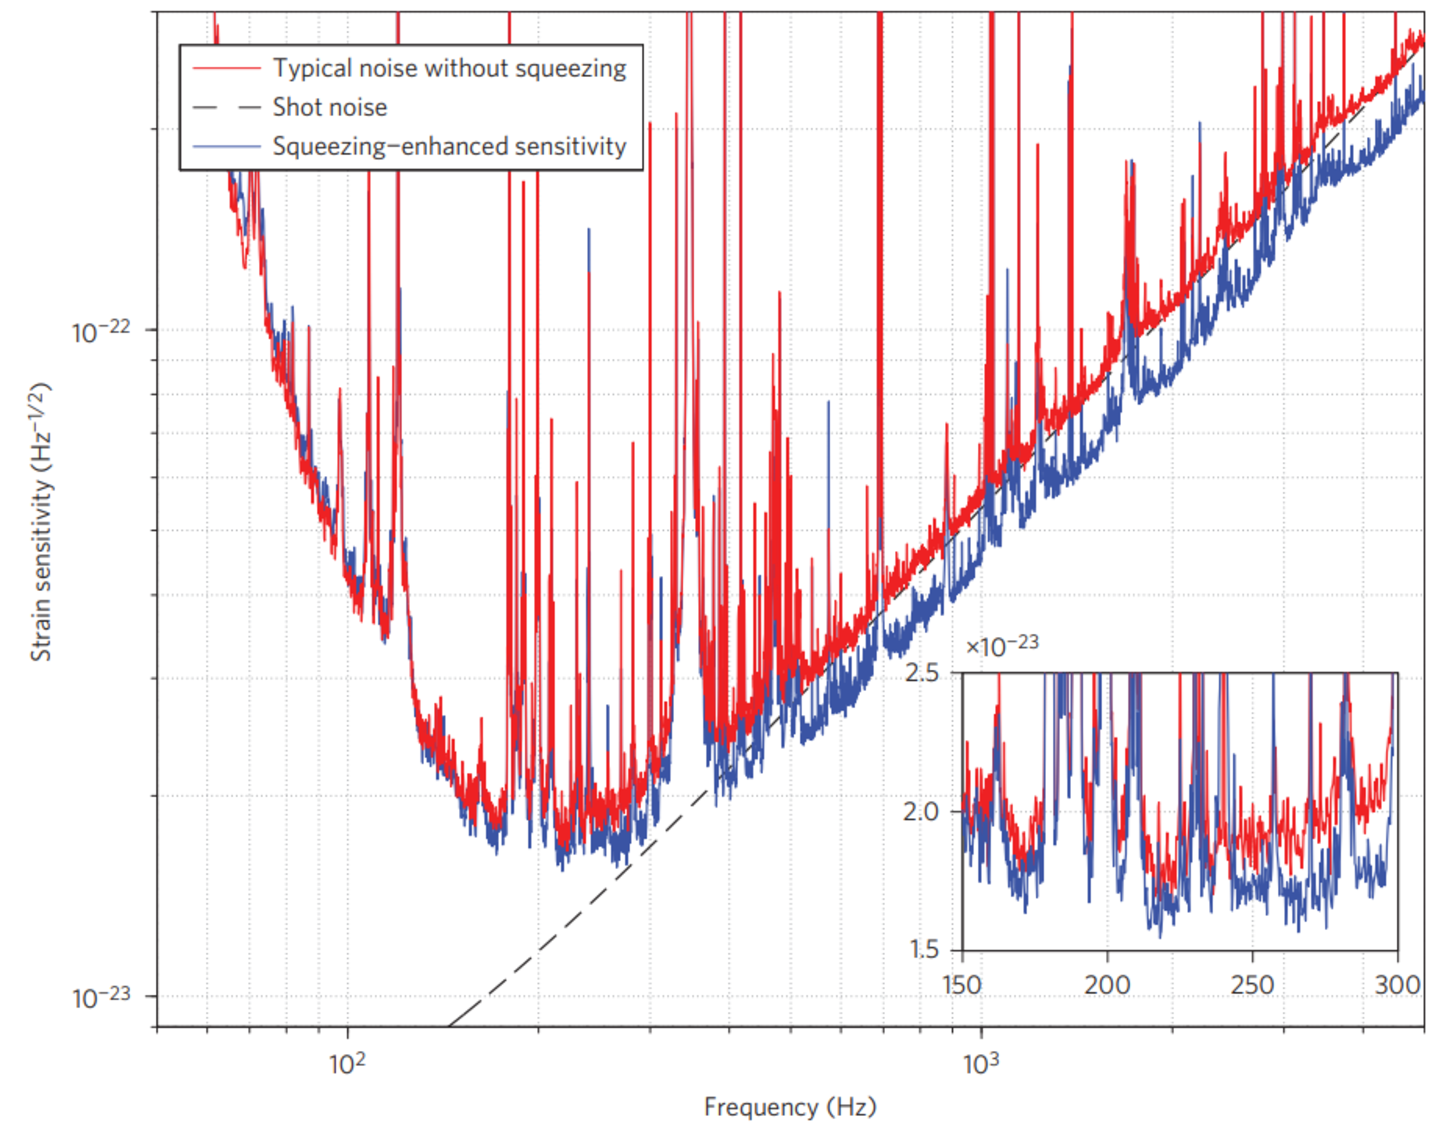
\includegraphics[width=0.8\textwidth]{L3/f10.pdf}
\caption{\justifying{在有和没有注入压缩态的情况下测量的H1探测器的应变灵敏度\citep{ref9}}}
\label{f10}
\end{figure}

\justifying{\setlength{\parindent}{2em}{图(\ref{f9})和图(\ref{f10})展示了压缩态光场注入激光干涉引力波探测器装置图和试验测试结果,可以看到注入压缩态后的实验结果和前述结果对应。}
%

\subsection{量子计算:实现量子逻辑门序列}

\justifying{\setlength{\parindent}{2em}{量子计算在解决大数分解、离散对数计算等难题中具有经典计算无法比拟的优势。任意高斯量子计算可以利用足够多的单模及双模基本逻辑门序列来实现。在此基础上,增加非高斯操作即可实现通用量子计算。在连续变量领域,cluster纠缠态是一种具有较高的纠缠保持特性的多组份纠缠态,其相互作用存在于相邻模式之间。山西大学量子光学与光量子器件国家重点实验室以连续变量六组份cluster纠缠态作为量子资源,完成了连续变量量子逻辑门序列的实验验证,它是由一个单模压缩操作和一个双模受控位相门组成的门序列\citep{ref10}。}
\begin{figure}[H]
\centering
	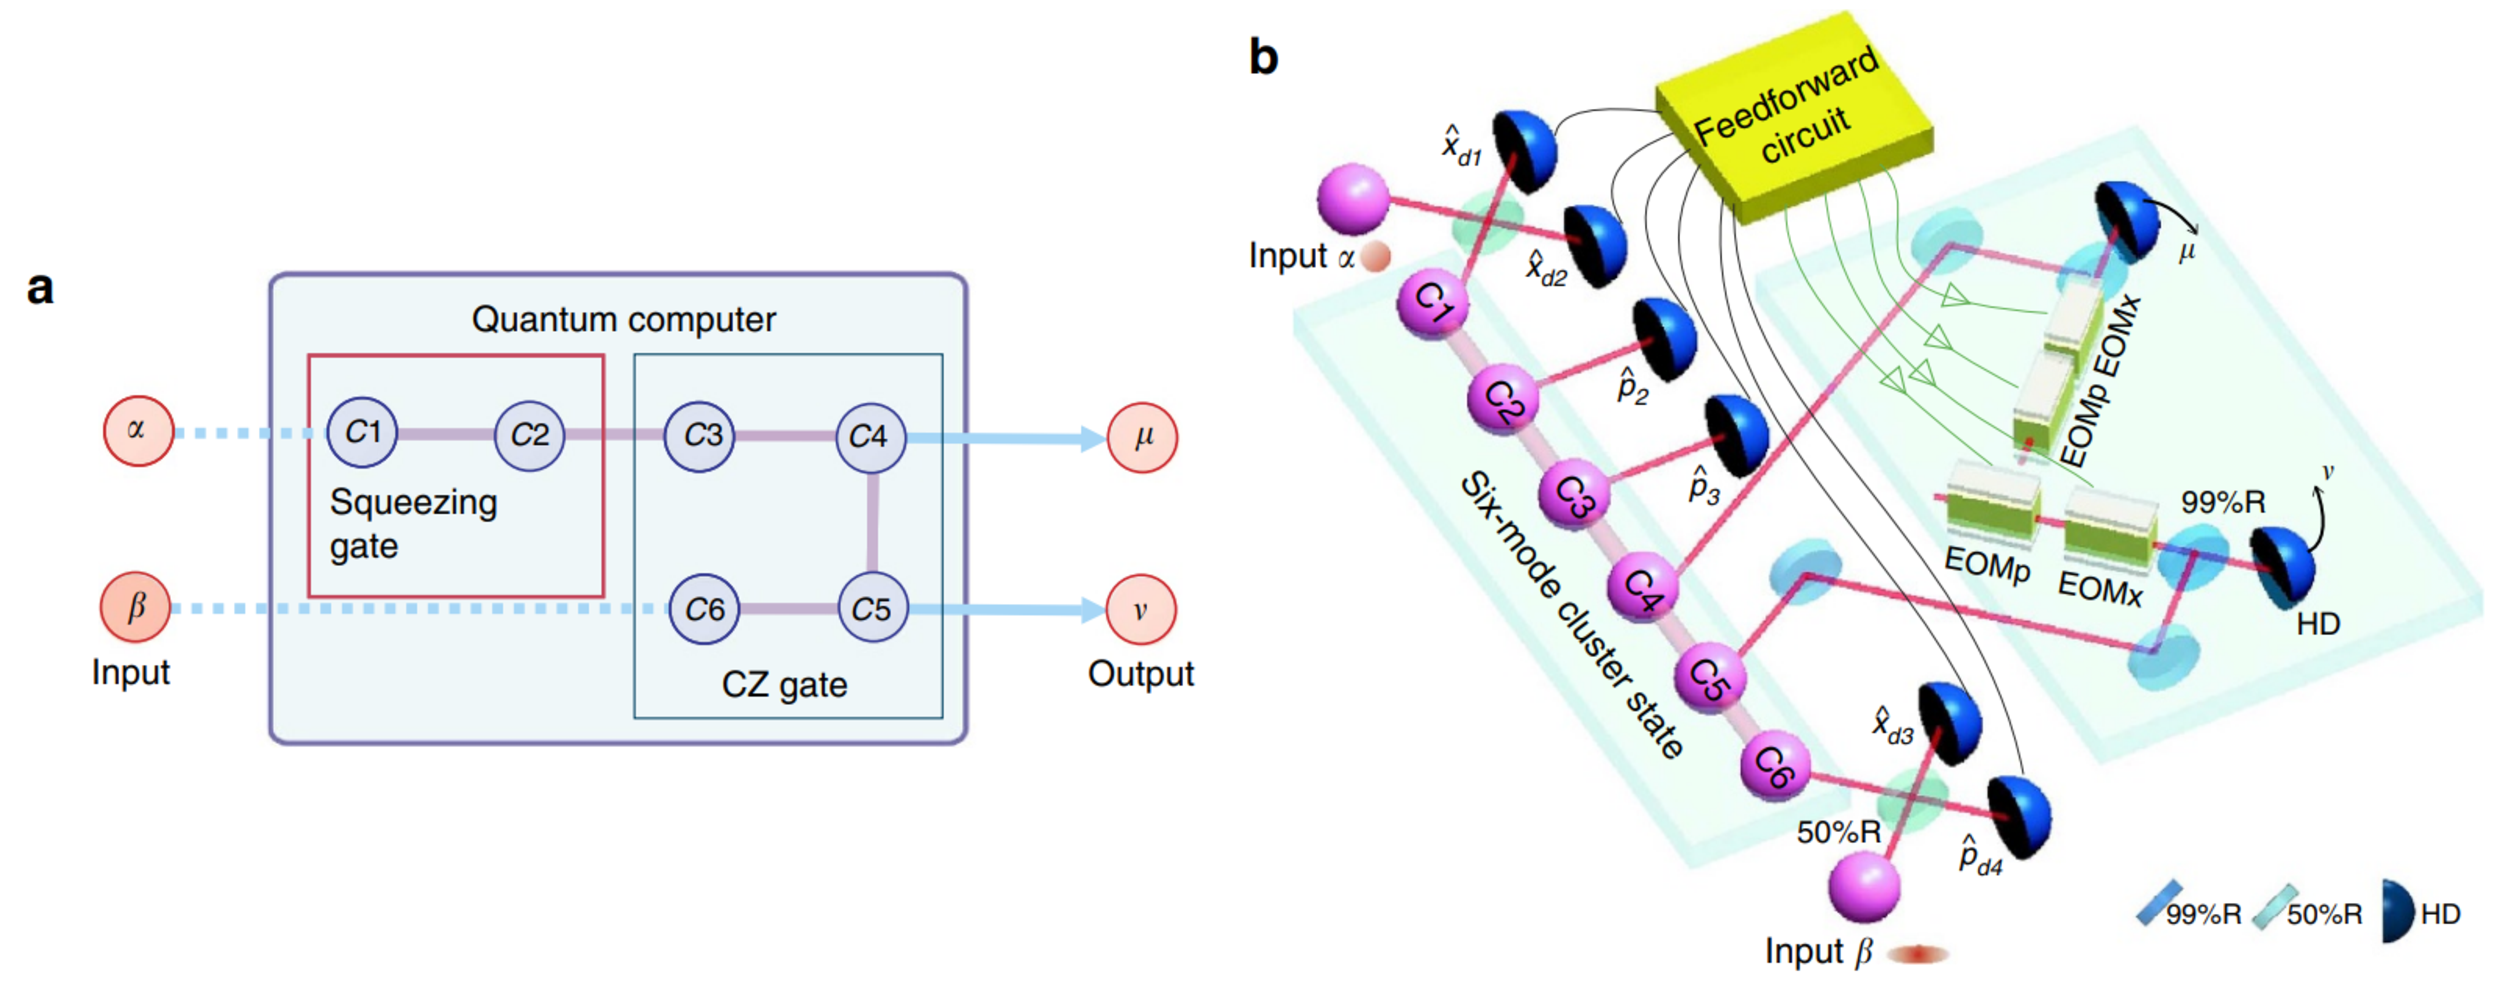
\includegraphics[width=0.9\textwidth]{L3/f11.pdf}
\caption{\justifying{利用连续变量 cluster态实现逻辑门序列的结构示意图\citep{ref10}}}
\label{f11}
\end{figure}

\justifying{\setlength{\parindent}{2em}{图(\ref{f11})为逻辑门序列的结构示意图和实验装置示意图。这个门序列的输出模式保真度和两个输出模式之间的纠缠度等量子特性在实验上得到了验证,输出模式之间的纠缠度既依赖于压缩门又依赖于受控位相门,因此验证了逻辑门的作用序列。该课题组提出的门序列方案可以扩展至更多逻辑门组合,为更复杂的通用多模高斯逻辑门序列提供了实验基础。}

\justifying{\setlength{\parindent}{2em}{压缩态光场也被应用于高斯玻色取样,与单光子态相比,压缩态光场的光子数分布本身的多样性进一步增强了高斯玻色采样的量子计算优势。2020年,中国科学技术大学潘建伟教授、陆朝阳教授课题组利用压缩态光场构建了“九章”量子计算系统,包含50个单模压缩态,输入一个100个入口、100个出口。近期,他们实现的“九章2.0”将干涉仪规模从之前的100个模式提升到了144个模式\citep{ref11}。}

\justifying{\setlength{\parindent}{2em}{当然,压缩态光场的应用还有很多,在精密测量方面有比如小吸收系数的测量、位移测量、位相测量等;在量子信息领域也有很多应用,基于高压缩度的纠缠态光场可以实现更远距离的量子隐形传态,利用集成光量子芯片制备压缩态光场能更好地实现量子纠错,使用压缩态光场可以实现量子增强的免标记受激拉曼散射等。}

\section{\large 小结/心得}

\justifying{\setlength{\parindent}{2em}{这个课设使我对光场压缩态有了一定的了解,在查阅参考资料的同时,我也了解到光场量子态不仅仅包括相干态、压缩态,还有热态、猫态、纠缠态等。当然,本文只是对单模(或简并)电磁场作了一定的压缩态理论分析,对双模电磁场的分析\citep{ref1,ref3,ref5}更为复杂就没有再展开分析了。}

\justifying{\setlength{\parindent}{2em}{在不违背海森堡不确定性关系的前提下,我们所了解的态从一般的量子态,到能够“稍微模糊”地确定电场振幅和相位的相干态,再到能够进一步通过压缩一个正交分量来实现精密测量的压缩态,再到后面一系列用于高保密通信的纠缠态等,这是一个循序渐进的过程,量子光学与量子信息领域逐渐发展了起来。我相信在不远的将来,光量子芯片能真正实现产业化,走遍千家万户,那将具有跨时代的意义。}

% 参考文献

\begin{thebibliography}{23}


\bibitem{ref1} %1
张智明.\sourcelink{book.douban.com/subject/30704757/}{量子光学}[M].北京:科学出版社,2015.

\bibitem{ref2} %2
秦忠忠,王美红,马荣,苏晓龙.\sourcelink{doi.org/10.3788/LOP202259.1100001}{压缩态光场及其应用研究进展}[J].激光与光电子学进展,2022,59(11):1100001.

\bibitem{ref3} %3
Gilbert Grynberg, Alain Aspect, Claude Fabre, and Claude Cohen-Tannoudji. \sourcelink{doi.org/10.1017/CBO9780511778261}{Introduction to quantum
optics from the semi-classical approach to quantized light}[M]. Cambridge University Press, 2012.

\bibitem{ref4} %4
Lvovsky A I. \sourcelink{doi.org/10.1002/9781119009719.ch5}{Squeezed light, photonics: scientific
foundations, technology and applications}[M]. Singapore:John Wiley \& Sons Inc, 2015: 121-163.

\bibitem{ref5} %5
谭维翰.\sourcelink{book.douban.com/subject/10738862/}{量子光学导论}[M].北京:科学出版社,2012.

\bibitem{ref6} %6
Corzo N, Marino A M, Jones K M, et al. \sourcelink{doi.org/10.1364/OE.19.021358}{Multispatial-mode single-beam quadrature squeezed states of light from four-wave mixing in hot rubidium vapor}[J]. Optics Express,2011,19(22):21358-21369.

\bibitem{ref7} %7
C. M. Caves. \sourcelink{journals.aps.org/prd/pdf/10.1103/PhysRevD.23.1693}{Quantum-mechanical Noise in an Interferometer}[J]. Physical Review D Particles\&Fields,1981,23(8):1693-1708.、

\bibitem{ref8} %8
要立婷.\sourcelink{kns.cnki.net/kcms/detail/detail.aspx?dbcode=CMFD&dbname=CMFD201801&filename=1017303380.nh&uniplatform=NZKPT&v=e7YWUBJogtind8GIHpm1aaaYTirlDbtsiGvwAQFGEG5vkz9gt8REPqYylDBSTt12}{光通信波段低频压缩态光场的产生及应用}[D].山西大学,2017.

\bibitem{ref9} %9
Aasi, J., Abadie, J., Abbott, B. et al. \sourcelink{doi.org/10.1038/nphoton.2013.177}{Enhanced sensitivity of the LIGO gravitational wave detector by using squeezed states of light}[J]. Nature Photonics,2013,7:613–619.

\bibitem{ref10} %10
Su X L, Hao S H, Deng X W, et al. \sourcelink{doi.org/10.1038/ncomms3828}{Gate sequence for continuous variable one-way quantum computation}[J]. Nature Communications,2013,4:2828.

\bibitem{ref11} %11
Zhong H S, Deng Y H, Qin J, et al. \sourcelink{journals.aps.org/prl/abstract/10.1103/PhysRevLett.127.180502}{Phaseprogrammable Gaussian boson sampling using stimulated squeezed light}[J]. Physical Review Letters,2021,127(18):180502.


\end{thebibliography}
\end{document}


